% Options for packages loaded elsewhere
\PassOptionsToPackage{unicode}{hyperref}
\PassOptionsToPackage{hyphens}{url}
%
\documentclass[
]{article}
\usepackage{amsmath,amssymb}
\usepackage{iftex}
\ifPDFTeX
  \usepackage[T1]{fontenc}
  \usepackage[utf8]{inputenc}
  \usepackage{textcomp} % provide euro and other symbols
\else % if luatex or xetex
  \usepackage{unicode-math} % this also loads fontspec
  \defaultfontfeatures{Scale=MatchLowercase}
  \defaultfontfeatures[\rmfamily]{Ligatures=TeX,Scale=1}
\fi
\usepackage{lmodern}
\ifPDFTeX\else
  % xetex/luatex font selection
\fi
% Use upquote if available, for straight quotes in verbatim environments
\IfFileExists{upquote.sty}{\usepackage{upquote}}{}
\IfFileExists{microtype.sty}{% use microtype if available
  \usepackage[]{microtype}
  \UseMicrotypeSet[protrusion]{basicmath} % disable protrusion for tt fonts
}{}
\makeatletter
\@ifundefined{KOMAClassName}{% if non-KOMA class
  \IfFileExists{parskip.sty}{%
    \usepackage{parskip}
  }{% else
    \setlength{\parindent}{0pt}
    \setlength{\parskip}{6pt plus 2pt minus 1pt}}
}{% if KOMA class
  \KOMAoptions{parskip=half}}
\makeatother
\usepackage{xcolor}
\usepackage[margin=1in]{geometry}
\usepackage{color}
\usepackage{fancyvrb}
\newcommand{\VerbBar}{|}
\newcommand{\VERB}{\Verb[commandchars=\\\{\}]}
\DefineVerbatimEnvironment{Highlighting}{Verbatim}{commandchars=\\\{\}}
% Add ',fontsize=\small' for more characters per line
\usepackage{framed}
\definecolor{shadecolor}{RGB}{248,248,248}
\newenvironment{Shaded}{\begin{snugshade}}{\end{snugshade}}
\newcommand{\AlertTok}[1]{\textcolor[rgb]{0.94,0.16,0.16}{#1}}
\newcommand{\AnnotationTok}[1]{\textcolor[rgb]{0.56,0.35,0.01}{\textbf{\textit{#1}}}}
\newcommand{\AttributeTok}[1]{\textcolor[rgb]{0.13,0.29,0.53}{#1}}
\newcommand{\BaseNTok}[1]{\textcolor[rgb]{0.00,0.00,0.81}{#1}}
\newcommand{\BuiltInTok}[1]{#1}
\newcommand{\CharTok}[1]{\textcolor[rgb]{0.31,0.60,0.02}{#1}}
\newcommand{\CommentTok}[1]{\textcolor[rgb]{0.56,0.35,0.01}{\textit{#1}}}
\newcommand{\CommentVarTok}[1]{\textcolor[rgb]{0.56,0.35,0.01}{\textbf{\textit{#1}}}}
\newcommand{\ConstantTok}[1]{\textcolor[rgb]{0.56,0.35,0.01}{#1}}
\newcommand{\ControlFlowTok}[1]{\textcolor[rgb]{0.13,0.29,0.53}{\textbf{#1}}}
\newcommand{\DataTypeTok}[1]{\textcolor[rgb]{0.13,0.29,0.53}{#1}}
\newcommand{\DecValTok}[1]{\textcolor[rgb]{0.00,0.00,0.81}{#1}}
\newcommand{\DocumentationTok}[1]{\textcolor[rgb]{0.56,0.35,0.01}{\textbf{\textit{#1}}}}
\newcommand{\ErrorTok}[1]{\textcolor[rgb]{0.64,0.00,0.00}{\textbf{#1}}}
\newcommand{\ExtensionTok}[1]{#1}
\newcommand{\FloatTok}[1]{\textcolor[rgb]{0.00,0.00,0.81}{#1}}
\newcommand{\FunctionTok}[1]{\textcolor[rgb]{0.13,0.29,0.53}{\textbf{#1}}}
\newcommand{\ImportTok}[1]{#1}
\newcommand{\InformationTok}[1]{\textcolor[rgb]{0.56,0.35,0.01}{\textbf{\textit{#1}}}}
\newcommand{\KeywordTok}[1]{\textcolor[rgb]{0.13,0.29,0.53}{\textbf{#1}}}
\newcommand{\NormalTok}[1]{#1}
\newcommand{\OperatorTok}[1]{\textcolor[rgb]{0.81,0.36,0.00}{\textbf{#1}}}
\newcommand{\OtherTok}[1]{\textcolor[rgb]{0.56,0.35,0.01}{#1}}
\newcommand{\PreprocessorTok}[1]{\textcolor[rgb]{0.56,0.35,0.01}{\textit{#1}}}
\newcommand{\RegionMarkerTok}[1]{#1}
\newcommand{\SpecialCharTok}[1]{\textcolor[rgb]{0.81,0.36,0.00}{\textbf{#1}}}
\newcommand{\SpecialStringTok}[1]{\textcolor[rgb]{0.31,0.60,0.02}{#1}}
\newcommand{\StringTok}[1]{\textcolor[rgb]{0.31,0.60,0.02}{#1}}
\newcommand{\VariableTok}[1]{\textcolor[rgb]{0.00,0.00,0.00}{#1}}
\newcommand{\VerbatimStringTok}[1]{\textcolor[rgb]{0.31,0.60,0.02}{#1}}
\newcommand{\WarningTok}[1]{\textcolor[rgb]{0.56,0.35,0.01}{\textbf{\textit{#1}}}}
\usepackage{graphicx}
\makeatletter
\def\maxwidth{\ifdim\Gin@nat@width>\linewidth\linewidth\else\Gin@nat@width\fi}
\def\maxheight{\ifdim\Gin@nat@height>\textheight\textheight\else\Gin@nat@height\fi}
\makeatother
% Scale images if necessary, so that they will not overflow the page
% margins by default, and it is still possible to overwrite the defaults
% using explicit options in \includegraphics[width, height, ...]{}
\setkeys{Gin}{width=\maxwidth,height=\maxheight,keepaspectratio}
% Set default figure placement to htbp
\makeatletter
\def\fps@figure{htbp}
\makeatother
\setlength{\emergencystretch}{3em} % prevent overfull lines
\providecommand{\tightlist}{%
  \setlength{\itemsep}{0pt}\setlength{\parskip}{0pt}}
\setcounter{secnumdepth}{-\maxdimen} % remove section numbering
\ifLuaTeX
  \usepackage{selnolig}  % disable illegal ligatures
\fi
\IfFileExists{bookmark.sty}{\usepackage{bookmark}}{\usepackage{hyperref}}
\IfFileExists{xurl.sty}{\usepackage{xurl}}{} % add URL line breaks if available
\urlstyle{same}
\hypersetup{
  pdftitle={Trabajo de Clasificación en Introducción a Ciencia de Datos. Dataset pima.},
  pdfauthor={Danel Arias},
  hidelinks,
  pdfcreator={LaTeX via pandoc}}

\title{Trabajo de Clasificación en Introducción a Ciencia de Datos.
Dataset pima.}
\author{Danel Arias}
\date{2023-12-11}

\begin{document}
\maketitle

\hypertarget{descripciuxf3n-del-trabajo}{%
\section{Descripción del trabajo}\label{descripciuxf3n-del-trabajo}}

El trabajo consiste en la realización de un análisis exploratorio de
datos (EDA) sobre un dataset y realizar una clasificación con diferentes
métodos para el dataset. El dataset indicado es el dataset pima, que
contiene datos sobre la diabetes de mujeres de la tribu pima.

\hypertarget{descripciuxf3n-del-dataset}{%
\section{Descripción del dataset}\label{descripciuxf3n-del-dataset}}

Según podemos leer en
\href{https://sci2s.ugr.es/keel/dataset.php?cod=21}{KEEL} se trata de un
dataset sobre la diabetes de los indios Pima extraido del Instituto
Nacional de Diabetes y Enfermedades Digestivas y Renales. Donde se
impusieron varias restricciones a la selección de estos casos de una
base de datos más amplia. En particular, todos los pacientes son mujeres
de al menos 21 años de ascendencia india Pima. La etiqueta de clase
representa si la persona tiene o no diabetes.

Las diferentes variables son:

\begin{itemize}
\tightlist
\item
  Preg: Número de veces que ha estado embarazada. {[}0-17{]}
\item
  Plas: Concentración plasmática de glucosa a las 2 horas en una prueba
  oral de tolerancia a la glucosa {[}0-199{]}
\item
  Pres: Presión arterial diastólica (mm Hg) {[}0-122{]}
\item
  Skin: Espesor del pliegue cutáneo del tríceps (mm) {[}0-99{]}
\item
  Insu: Insulina sérica de 2 horas (mu U/ml) {[}0-846{]}
\item
  Mass: Índice de masa corporal (peso en kg/(altura en m)\^{}2)
  {[}0-67.1{]}
\item
  Pedi: Función de pedigrí de la diabetes {[}0.078-2.42{]}
\item
  Age: Edad (años) {[}21-81{]}
\item
  Class: Variable de clase (`tested\_negative' o `tested\_positive')
\end{itemize}

En total el dataset tiene 8 variables y 768 observaciones. Además, según
la descripción en KEEL este dataset no contiene valores perdidos (NA's).

\hypertarget{preparaciuxf3n-inicial-del-entorno}{%
\section{Preparación inicial del
entorno}\label{preparaciuxf3n-inicial-del-entorno}}

\hypertarget{carga-de-libreruxedas}{%
\subsection{Carga de librerías}\label{carga-de-libreruxedas}}

\begin{Shaded}
\begin{Highlighting}[]
\FunctionTok{library}\NormalTok{(ggplot2)}
\FunctionTok{library}\NormalTok{(moments)}
\FunctionTok{library}\NormalTok{(corrplot)}
\FunctionTok{library}\NormalTok{(dplyr)}
\FunctionTok{library}\NormalTok{(caret)}
\FunctionTok{library}\NormalTok{(class)}
\FunctionTok{library}\NormalTok{(MASS)}
\FunctionTok{library}\NormalTok{(tidyverse)}
\FunctionTok{library}\NormalTok{(ggthemes)}
\FunctionTok{library}\NormalTok{(gridExtra)}
\FunctionTok{library}\NormalTok{(klaR)}
\end{Highlighting}
\end{Shaded}

\hypertarget{carga-de-datos}{%
\subsection{Carga de datos}\label{carga-de-datos}}

Cargamos los datos de pima/pima.dat. Al ser un fichero .dat debemos
obviar las filas que no son datos, estas empiezan en `@'

\begin{Shaded}
\begin{Highlighting}[]
\NormalTok{pima }\OtherTok{\textless{}{-}} \FunctionTok{read.table}\NormalTok{(}\StringTok{"pima/pima.dat"}\NormalTok{, }\AttributeTok{header =} \ConstantTok{FALSE}\NormalTok{,}
                   \AttributeTok{sep =} \StringTok{","}\NormalTok{, }\AttributeTok{comment.char =} \StringTok{"@"}\NormalTok{)}
\end{Highlighting}
\end{Shaded}

Añadimos los nombres de las columnas. Los nombres de las columnas están
en pima.dat. Y se encuentran en la línea tras `@inputs' así que lo
leemos y lo añadimos.

\begin{Shaded}
\begin{Highlighting}[]
\NormalTok{nombres }\OtherTok{\textless{}{-}} \FunctionTok{grep}\NormalTok{(}\StringTok{"\^{}@inputs"}\NormalTok{, }\FunctionTok{readLines}\NormalTok{(}\StringTok{"pima/pima.dat"}\NormalTok{), }\AttributeTok{value =} \ConstantTok{TRUE}\NormalTok{) }\SpecialCharTok{\%\textgreater{}\%} 
  \CommentTok{\# Eliminamos el @inputs}
  \FunctionTok{str\_remove}\NormalTok{(}\StringTok{"@inputs "}\NormalTok{) }\SpecialCharTok{\%\textgreater{}\%} 
  \CommentTok{\#Eliminamos espacions}
  \FunctionTok{str\_remove\_all}\NormalTok{(}\StringTok{" "}\NormalTok{) }\SpecialCharTok{\%\textgreater{}\%}
  \CommentTok{\# Separamos por comas}
  \FunctionTok{str\_split}\NormalTok{(}\StringTok{","}\NormalTok{) }\SpecialCharTok{\%\textgreater{}\%} 
  \CommentTok{\# Convertimos a vector}
  \FunctionTok{unlist}\NormalTok{()}

\CommentTok{\# El nombre de la última variable se encuentra tras @outputs}
\NormalTok{nombre\_output }\OtherTok{\textless{}{-}} \FunctionTok{grep}\NormalTok{(}\StringTok{"\^{}@outputs"}\NormalTok{, }\FunctionTok{readLines}\NormalTok{(}\StringTok{"pima/pima.dat"}\NormalTok{), }\AttributeTok{value =} \ConstantTok{TRUE}\NormalTok{) }\SpecialCharTok{\%\textgreater{}\%} 
  \CommentTok{\# Eliminamos el @outputs}
  \FunctionTok{str\_remove}\NormalTok{(}\StringTok{"@outputs "}\NormalTok{)}

\CommentTok{\# Añadimos el nombre de la última variable}
\NormalTok{nombres }\OtherTok{\textless{}{-}} \FunctionTok{c}\NormalTok{(nombres, nombre\_output)}

\CommentTok{\# Añadimos los nombres al dataset}
\FunctionTok{colnames}\NormalTok{(pima) }\OtherTok{\textless{}{-}}\NormalTok{ nombres}
\end{Highlighting}
\end{Shaded}

\hypertarget{anuxe1lisis-exploratorio-de-datos}{%
\section{Análisis exploratorio de
datos}\label{anuxe1lisis-exploratorio-de-datos}}

Primero echamos un vistazo a los datos son un \texttt{summary()}.
Podemos ver que cuadra con la descripción proporcionada.

\begin{verbatim}
##       Preg             Plas            Pres             Skin      
##  Min.   : 0.000   Min.   :  0.0   Min.   :  0.00   Min.   : 0.00  
##  1st Qu.: 1.000   1st Qu.: 99.0   1st Qu.: 62.00   1st Qu.: 0.00  
##  Median : 3.000   Median :117.0   Median : 72.00   Median :23.00  
##  Mean   : 3.845   Mean   :120.9   Mean   : 69.11   Mean   :20.54  
##  3rd Qu.: 6.000   3rd Qu.:140.2   3rd Qu.: 80.00   3rd Qu.:32.00  
##  Max.   :17.000   Max.   :199.0   Max.   :122.00   Max.   :99.00  
##       Insu            Mass            Pedi             Age       
##  Min.   :  0.0   Min.   : 0.00   Min.   :0.0780   Min.   :21.00  
##  1st Qu.:  0.0   1st Qu.:27.30   1st Qu.:0.2437   1st Qu.:24.00  
##  Median : 30.5   Median :32.00   Median :0.3725   Median :29.00  
##  Mean   : 79.8   Mean   :31.99   Mean   :0.4719   Mean   :33.24  
##  3rd Qu.:127.2   3rd Qu.:36.60   3rd Qu.:0.6262   3rd Qu.:41.00  
##  Max.   :846.0   Max.   :67.10   Max.   :2.4200   Max.   :81.00  
##     Class          
##  Length:768        
##  Class :character  
##  Mode  :character  
##                    
##                    
## 
\end{verbatim}

Revisamos si tenemos NA's por si acaso y confirmamos lo que se nos
indicaba en KEEL, no hay NA's.

\begin{Shaded}
\begin{Highlighting}[]
\FunctionTok{colSums}\NormalTok{(}\FunctionTok{is.na}\NormalTok{(pima))}
\end{Highlighting}
\end{Shaded}

\begin{verbatim}
##  Preg  Plas  Pres  Skin  Insu  Mass  Pedi   Age Class 
##     0     0     0     0     0     0     0     0     0
\end{verbatim}

\hypertarget{anuxe1lisis-variable-a-variable}{%
\subsection{Análisis variable a
variable}\label{anuxe1lisis-variable-a-variable}}

En este apartado analizaremos cada variable por separado.

\hypertarget{variable-class}{%
\subsubsection{Variable `Class'}\label{variable-class}}

Comezamos con la variable `Class' que es una variable categórica
binaria. La convertimos a factor para poder trabajar con ella y
visualizamos los valores que toma (Figura \ref{fig:bar_class}) donde
vemos que hay más mujeres que no tienen diabetes que mujeres que sí la
tienen.

\begin{figure}

{\centering 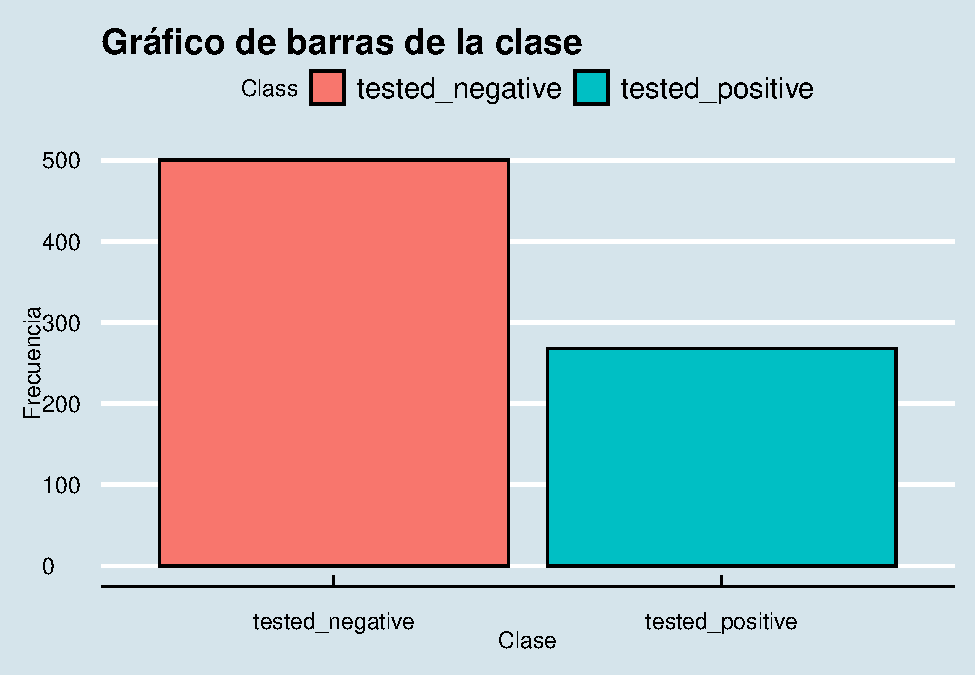
\includegraphics[width=0.5\linewidth]{pima-clasificacion_files/figure-latex/bar_class-1} 

}

\caption{ Gráfico de barras de la clase}\label{fig:bar_class}
\end{figure}

\hypertarget{variable-preg}{%
\subsubsection{Variable `Preg'}\label{variable-preg}}

Para comenzar con las variables numéricas estudiamos la variable `Preg'.
Sabemos que pertenece al rango {[}0-17{]}. Para más detalle, vemos un
histograma en la Figura (\ref{fig:hist_preg}). Vemos que hay un gran
número de mujeres que no han estado embarazadas, y que el número de
embarazos va disminuyendo conforme aumenta el número de embarazos.

\begin{figure}

{\centering 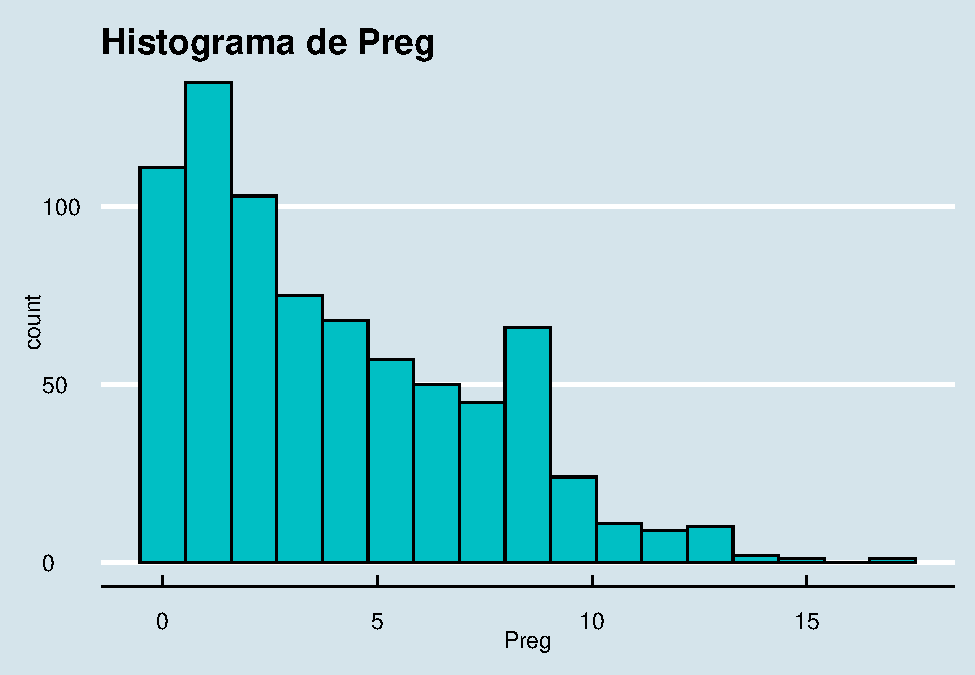
\includegraphics[width=0.5\linewidth]{pima-clasificacion_files/figure-latex/hist_preg-1} 

}

\caption{Histograma de Preg}\label{fig:hist_preg}
\end{figure}

Estudiamos también los cuantiles con un boxplot (Figura
\ref{fig:box_preg}). Donde vemos que el 25\% de las mujeres no han
estado embarazadas y y que solo un 25\% ha estado embarazada más de 6
veces. Observamos que hay valores atípicos principalmente en el extremo
superior, estos parecen ser valores correctos, por lo que no los
eliminaremos.

\begin{verbatim}
##   0%  25%  50%  75% 100% 
##    0    1    3    6   17
\end{verbatim}

\begin{figure}

{\centering 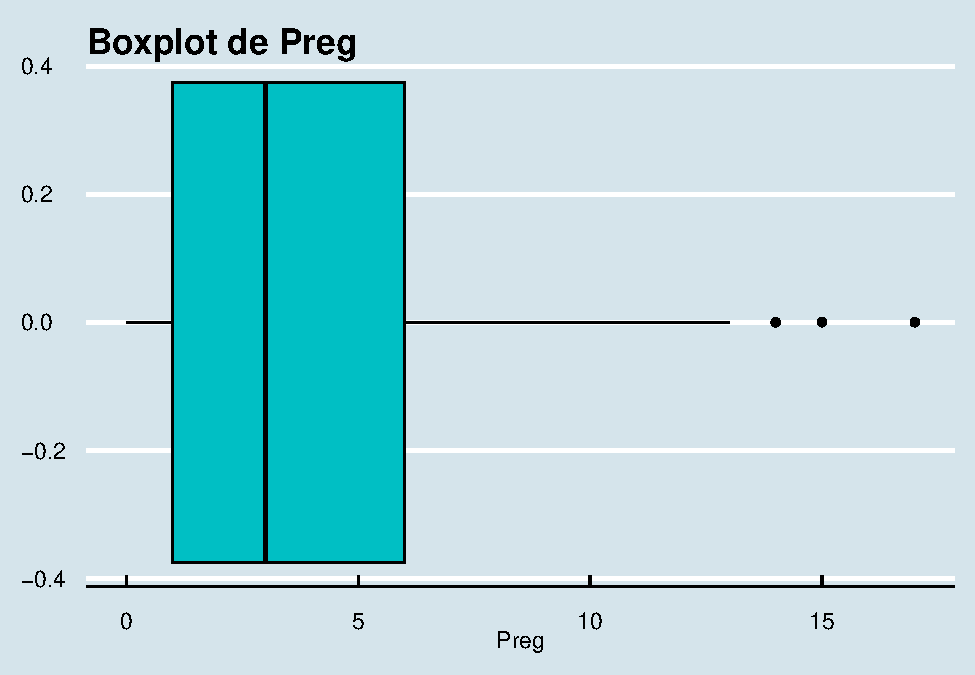
\includegraphics[width=0.5\linewidth]{pima-clasificacion_files/figure-latex/box_preg-1} 

}

\caption{Boxplot de Preg}\label{fig:box_preg}
\end{figure}

Estudiamos la forma de la variable Preg. Para ello miramos la media, sd,
skewness y kurtosis.

\begin{verbatim}
## [1] "Media: 3.8451"
\end{verbatim}

\begin{verbatim}
## [1] "Deviación estándar: 3.3696"
\end{verbatim}

Para estudiar la skewness y la kurtosis usaremos los tests de D'Agostino
y Anscombe respectivamente.

\begin{verbatim}
## [1] "Skewness: 0.8999"
\end{verbatim}

\begin{verbatim}
## 
##  D'Agostino skewness test
## 
## data:  pima$Preg
## skew = 0.89991, z = 8.90464, p-value < 2.2e-16
## alternative hypothesis: data have a skewness
\end{verbatim}

Dado que la skewness \textgreater{} 0 la distribución está sesgada a la
derecha. Ademas el valor de p-value del test de D'agostino es menor que
0.05, por lo que podemos afirmar con seguridad que la distribución está
sesgada a la derecha.

\begin{verbatim}
## [1] "Kurtosis: 3.1504"
\end{verbatim}

\begin{verbatim}
## 
##  Anscombe-Glynn kurtosis test
## 
## data:  pima$Preg
## kurt = 3.15038, z = 0.93339, p-value = 0.3506
## alternative hypothesis: kurtosis is not equal to 3
\end{verbatim}

Dados que la kurtosis \textgreater{} 0 la distribución tiene colas
pesadas. En cambio el valor de p-value del test de Anscombe es mayor que
0.05, por lo que es posible que no se pueda afirmar que la distribución
no es normal. Podemos verlo mejor con gráfico de densidad (ver Figura
\ref{fig:densidad_preg}). Realizamos el test de Shapiro-Wilk para
confirmar la normalidad de la variable. Donde vemos que el valor de
p-value es menor que 0.05, por lo que la variable Preg no sigue una
distribución normal. Lo vemos también el QQ-plot (Figura
\ref{fig:qq_preg}).

\begin{verbatim}
## 
##  Shapiro-Wilk normality test
## 
## data:  pima$Preg
## W = 0.90428, p-value < 2.2e-16
\end{verbatim}

\begin{figure}

{\centering 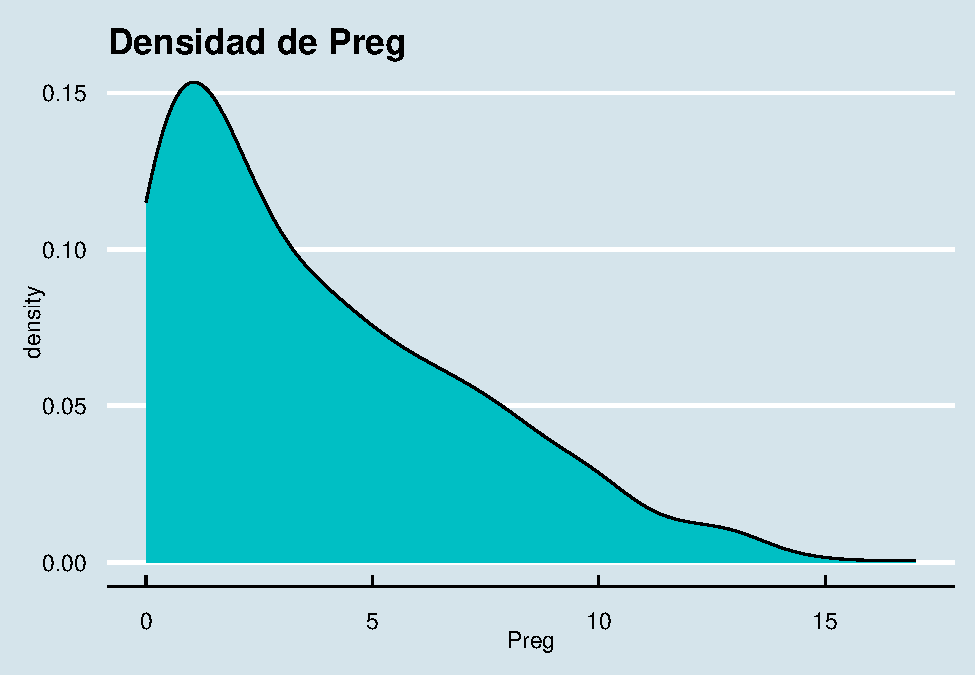
\includegraphics[width=0.5\linewidth]{pima-clasificacion_files/figure-latex/densidad_preg-1} 

}

\caption{Densidad de Preg}\label{fig:densidad_preg}
\end{figure}

\begin{figure}

{\centering 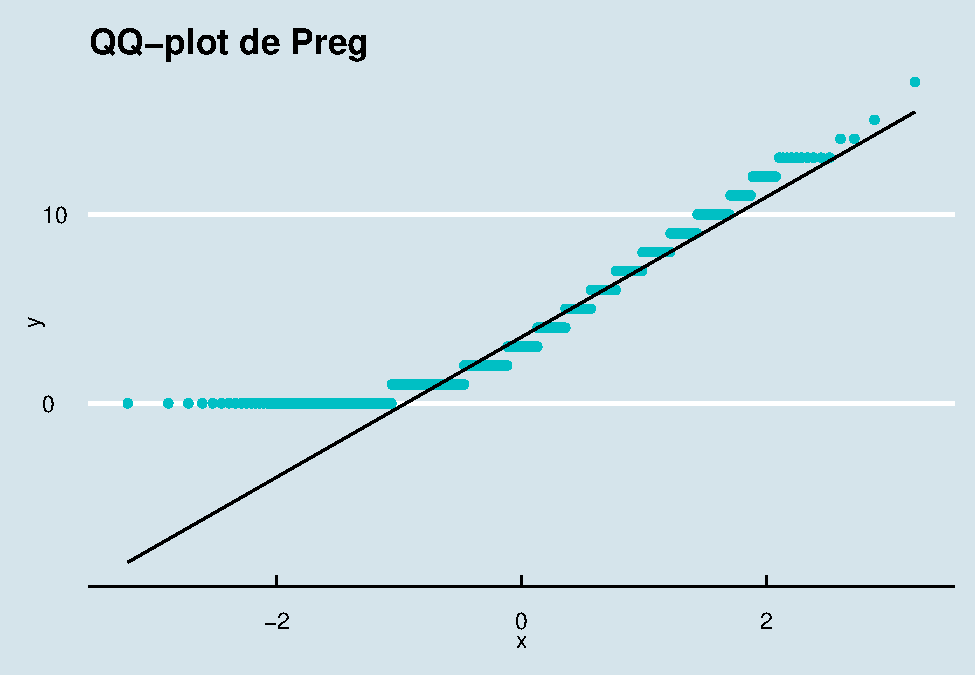
\includegraphics[width=0.5\linewidth]{pima-clasificacion_files/figure-latex/qq_preg-1} 

}

\caption{QQ-plot de Preg}\label{fig:qq_preg}
\end{figure}

\hypertarget{variable-plas}{%
\subsubsection{Variable `Plas'}\label{variable-plas}}

Estudiamos la variable `Plas' perteneciente al rango {[}0-199{]}. Para
más detalle, vemos un histograma en la Figura (\ref{fig:hist_plas}).
Vemos que hay un gran número de mujeres con una concentración de glucosa
en plasma entre 80 y 130.

\begin{figure}

{\centering 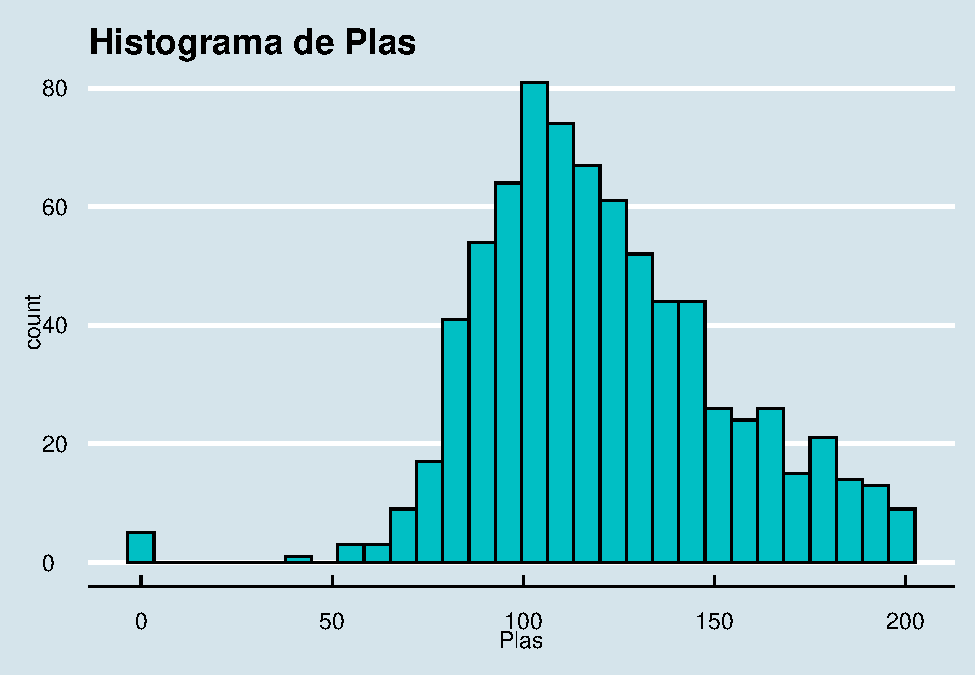
\includegraphics[width=0.5\linewidth]{pima-clasificacion_files/figure-latex/hist_plas-1} 

}

\caption{Histograma de Plas}\label{fig:hist_plas}
\end{figure}

Llama la atención que haya un pequeño pico en 0, esto puede indicar que
hay valores perdidos. Dada la naturaleza de la variable, la
concentración plasmática de glucosa no puede ser 0. Asignamos estos
valores como NA's y toca valorar como imputarlos. Dado que son pocos
valores y que la distribución es bastante simétrica, imputaremos con la
media.

\begin{verbatim}
## [1] "Resumen antes de imputar:"
\end{verbatim}

\begin{verbatim}
##    Min. 1st Qu.  Median    Mean 3rd Qu.    Max.    NA's 
##    44.0    99.0   117.0   121.7   141.0   199.0       5
\end{verbatim}

\begin{verbatim}
## [1] "Resumen después de imputar:"
\end{verbatim}

\begin{verbatim}
##    Min. 1st Qu.  Median    Mean 3rd Qu.    Max. 
##   44.00   99.75  117.00  121.69  140.25  199.00
\end{verbatim}

Estudiamos también los cuantiles con un boxplot (Figura
\ref{fig:box_plas}). Donde se observa que el 25\% de las mujeres tienen
una concentración de glucosa en plasma menor de 100, y que el 25\% de
las mujeres tienen una concentración de glucosa en plasma mayor de 140.

\begin{verbatim}
##     0%    25%    50%    75%   100% 
##  44.00  99.75 117.00 140.25 199.00
\end{verbatim}

\begin{figure}

{\centering 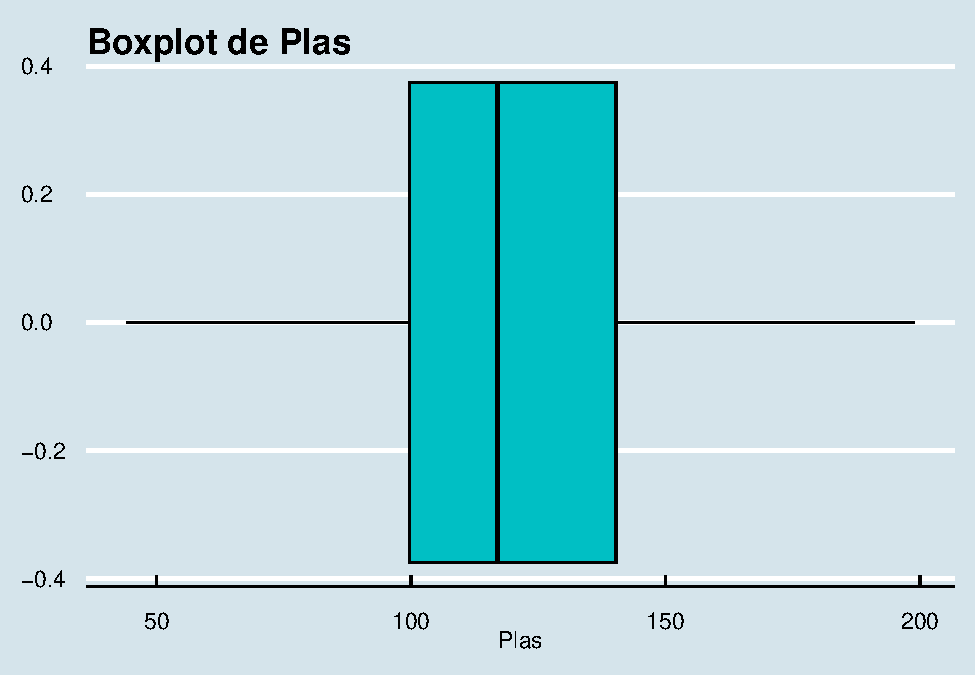
\includegraphics[width=0.5\linewidth]{pima-clasificacion_files/figure-latex/box_plas-1} 

}

\caption{Boxplot de Plas}\label{fig:box_plas}
\end{figure}

Estudiamos la forma de la variable Plas, Para ello miramos la media, sd,
skewness y kurtosis.

\begin{verbatim}
## [1] "Media: 121.6868"
\end{verbatim}

\begin{verbatim}
## [1] "Deviación estándar: 30.4359"
\end{verbatim}

Para estudiar la skewness y la kurtosis usaremos los tests de D'Agostino
y Anscombe respectivamente.

\begin{verbatim}
## [1] "Skewness: 0.5317"
\end{verbatim}

\begin{verbatim}
## 
##  D'Agostino skewness test
## 
## data:  pima$Plas
## skew = 0.53168, z = 5.71818, p-value = 1.077e-08
## alternative hypothesis: data have a skewness
\end{verbatim}

Dado que skewness \textgreater{} 0 la distribución está sesgada a la
derecha. Además el valor de p-value del test de D'agostino es menor que
0.05, por lo que podemos afirmar con seguridad que la distribución está
sesgada a la derecha.

\begin{verbatim}
## [1] "Kurtosis: 2.7347"
\end{verbatim}

\begin{verbatim}
## 
##  Anscombe-Glynn kurtosis test
## 
## data:  pima$Plas
## kurt = 2.7347, z = -1.6211, p-value = 0.105
## alternative hypothesis: kurtosis is not equal to 3
\end{verbatim}

Dado que kurtosis \textgreater{} 0 la distribución tiene colas pesadas.
En cambio el valor de p-value del test de Anscombe es mayor que 0.05,
por lo que no se puede afirmar que la distribución no es normal.
Visualizamos esto mejor con un gráfico de densidad (ver Figura
\ref{fig:densidad_plas}) donde no se ve claramente que la distribución
rechaze la normalidad. Por lo tanto realizamos el test de Shapiro-Wilk
para ver si la variable Plas sigue una distribución normal y para
visualizarlo mejor usamos un QQ-plot (ver Figura \ref{fig:qq_plas}). El
valor de p-value es menor que 0.05, por lo que podemos afirmar que la
variable Plas no sigue una distribución normal.

\begin{verbatim}
## 
##  Shapiro-Wilk normality test
## 
## data:  pima$Plas
## W = 0.9699, p-value = 1.777e-11
\end{verbatim}

\begin{figure}

{\centering 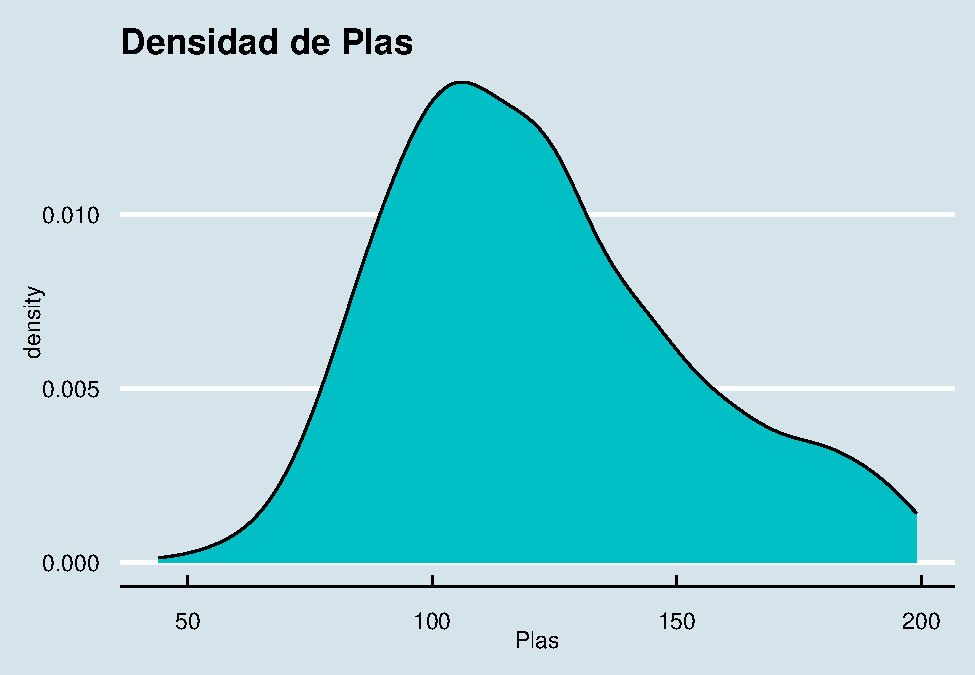
\includegraphics[width=0.5\linewidth]{pima-clasificacion_files/figure-latex/densidad_plas-1} 

}

\caption{Densidad de Plas}\label{fig:densidad_plas}
\end{figure}

\begin{figure}

{\centering 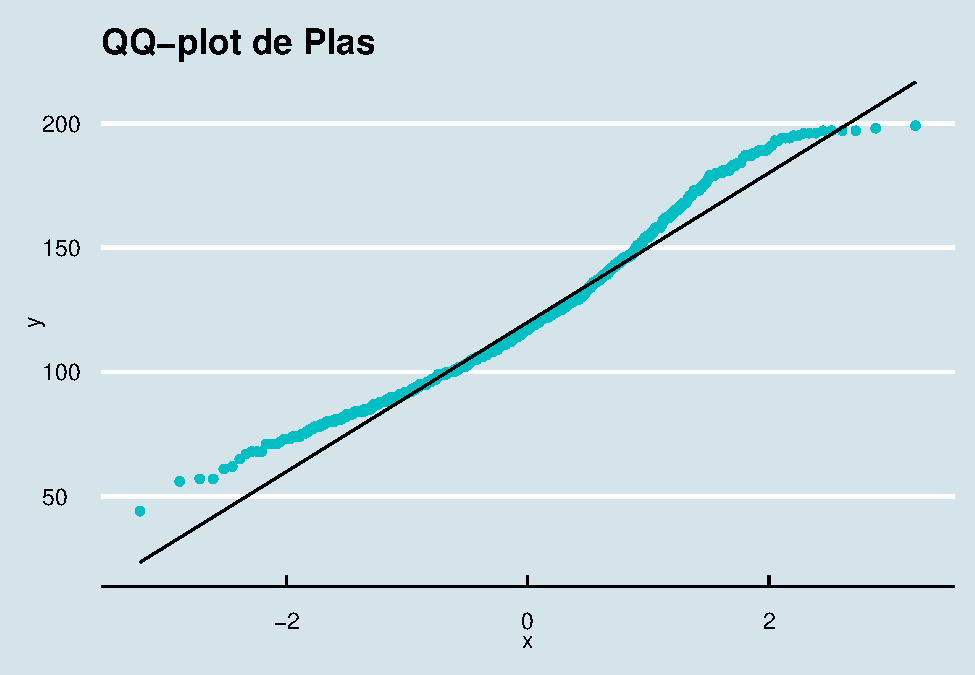
\includegraphics[width=0.5\linewidth]{pima-clasificacion_files/figure-latex/qq_plas-1} 

}

\caption{QQ-plot de Plas}\label{fig:qq_plas}
\end{figure}

\hypertarget{variable-pres}{%
\subsubsection{Variable `Pres'}\label{variable-pres}}

Estudiamos a continuación la variable `Pres' que se refiere a la presión
arterial diastólica la cual pertenece al rango {[}0, 122{]}.
Visualizamos la distribución de la variable con un histograma (Figura
\ref{fig:hist_pres}). Donde vemos que la mayoría de los valores se
encuentran entre 40 y 100, y que hay un pico en 0.

\begin{figure}

{\centering 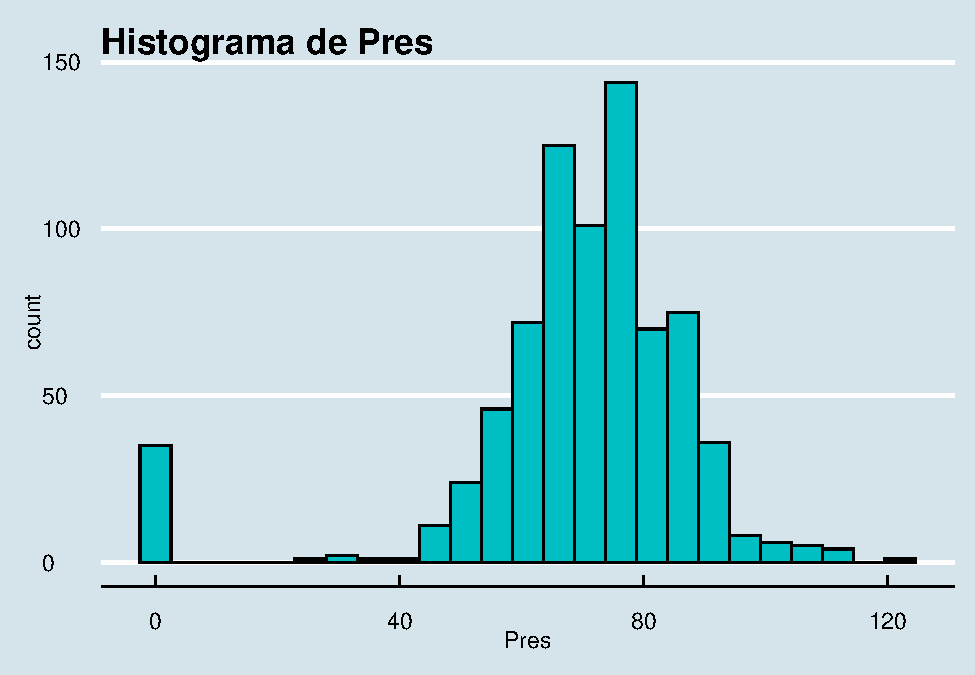
\includegraphics[width=0.5\linewidth]{pima-clasificacion_files/figure-latex/hist_pres-1} 

}

\caption{Histograma de Pres}\label{fig:hist_pres}
\end{figure}

El pico en el valor 0 es interesante ya que puede indicar que hay
valores perdidos. Dada la naturaleza de la variable, la presión arterial
diastólica no puede ser 0. Asignamos estos valores como NA's y toca
valorar como imputarlos. Dado que son pocos valores y que la
distribución es bastante simétrica, imputaremos con la media.

\begin{verbatim}
## [1] "Resumen antes de imputar:"
\end{verbatim}

\begin{verbatim}
##    Min. 1st Qu.  Median    Mean 3rd Qu.    Max.    NA's 
##   24.00   64.00   72.00   72.41   80.00  122.00      35
\end{verbatim}

\begin{verbatim}
## [1] "Resumen después de imputar:"
\end{verbatim}

\begin{verbatim}
##    Min. 1st Qu.  Median    Mean 3rd Qu.    Max. 
##   24.00   64.00   72.20   72.41   80.00  122.00
\end{verbatim}

Estudiamos también los cuantiles con un boxplot (Figura
\ref{fig:box_pres}) y vemos que el 25\% de las mujeres tienen una
presión arterial diastólica menor de 64, y que el 25\% de las mujeres
tienen una presión arterial diastólica mayor de 80.

\begin{verbatim}
##        0%       25%       50%       75%      100% 
##  24.00000  64.00000  72.20259  80.00000 122.00000
\end{verbatim}

\begin{figure}

{\centering 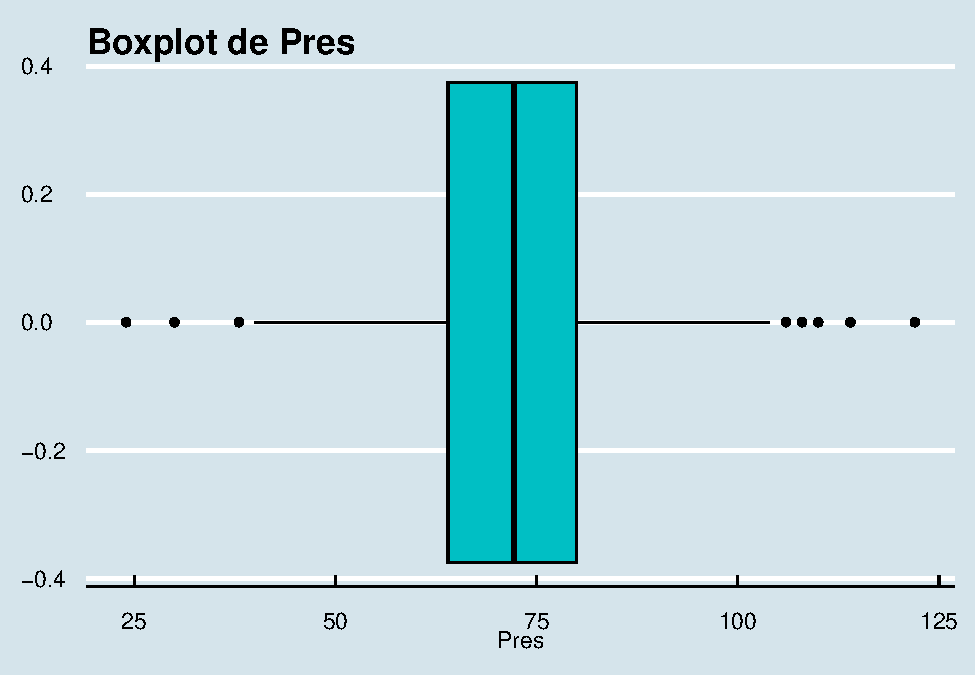
\includegraphics[width=0.5\linewidth]{pima-clasificacion_files/figure-latex/box_pres-1} 

}

\caption{Boxplot de Pres}\label{fig:box_pres}
\end{figure}

Estudiamos la forma de la variable Pres.~Para ello miramos la media, sd,
skewness y kurtosis.

\begin{verbatim}
## [1] "Media: 72.4052"
\end{verbatim}

\begin{verbatim}
## [1] "Desviación estándar: 12.0963"
\end{verbatim}

Para estudiar la skewness y la kurtosis usaremos los tests de D'Agostino
y Anscombe respectivamente.

\begin{verbatim}
## [1] "Skewness: 0.137"
\end{verbatim}

\begin{verbatim}
## 
##  D'Agostino skewness test
## 
## data:  pima$Pres
## skew = 0.13704, z = 1.55814, p-value = 0.1192
## alternative hypothesis: data have a skewness
\end{verbatim}

Dados que skewness \textgreater{} 0 la distribución está sesgada a la
derecha. En cambio el valor de p-value del test de D'agostino es mayor
que 0.05, por lo que no podemos afirmar con seguridad que la
distribución este sesgada.

\begin{verbatim}
## [1] "Kurtosis: 4.0828"
\end{verbatim}

\begin{verbatim}
## 
##  Anscombe-Glynn kurtosis test
## 
## data:  pima$Pres
## kurt = 4.0828, z = 4.2911, p-value = 1.778e-05
## alternative hypothesis: kurtosis is not equal to 3
\end{verbatim}

Dado que kurtosis \textgreater{} 0 la distribución tiene colas pesadas.
Además el valor de p-value del test de Anscombe es menor que 0.05, por
lo que podemos afirmar con seguridad que la distribución no es normal.
Podemos verlo mejor con un gráfico de densidad (Figura
\ref{fig:densidad_pres}). Estudiamos de todas formas la normalidad de la
variable Pres con el test de Shapiro-Wilk y lo visualizamos con un
QQ-plot (Figura \ref{fig:qq_pres}).

\begin{verbatim}
## 
##  Shapiro-Wilk normality test
## 
## data:  pima$Pres
## W = 0.98804, p-value = 6.463e-06
\end{verbatim}

\begin{figure}

{\centering 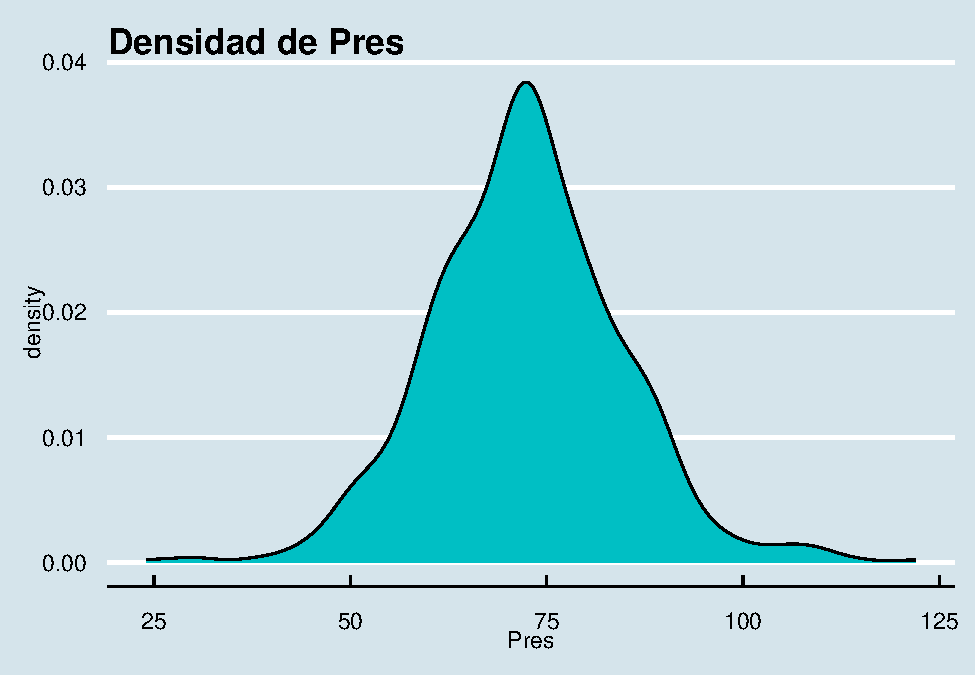
\includegraphics[width=0.5\linewidth]{pima-clasificacion_files/figure-latex/densidad_pres-1} 

}

\caption{Densidad de Pres}\label{fig:densidad_pres}
\end{figure}
\begin{figure}

{\centering 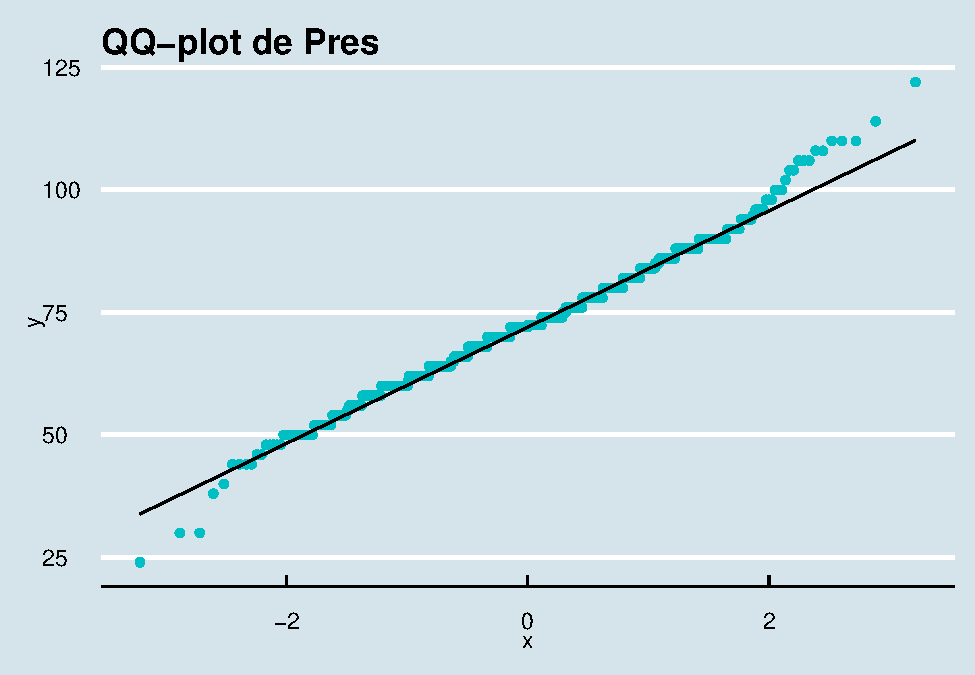
\includegraphics[width=0.5\linewidth]{pima-clasificacion_files/figure-latex/qq_pres-1} 

}

\caption{QQ-plot de Pres}\label{fig:qq_pres}
\end{figure}

\hypertarget{variable-skin}{%
\subsubsection{Variable `Skin'}\label{variable-skin}}

Ahora la variable `Skin' que se refiere al grosor del pliegue cutáneo
del tríceps. Vemos que los valores pertenecen al rango {[}0-99{]}, para
más detalle vamos a ver el histograma (Figura \ref{fig:hist_skin}).
Vemos que el grueso de los valores se encuentran entre 5 y 60, con un
gran pico en 0 y con un pequeño pico en 100. Esto puede indicar que hay
valores perdidos,

\begin{figure}

{\centering 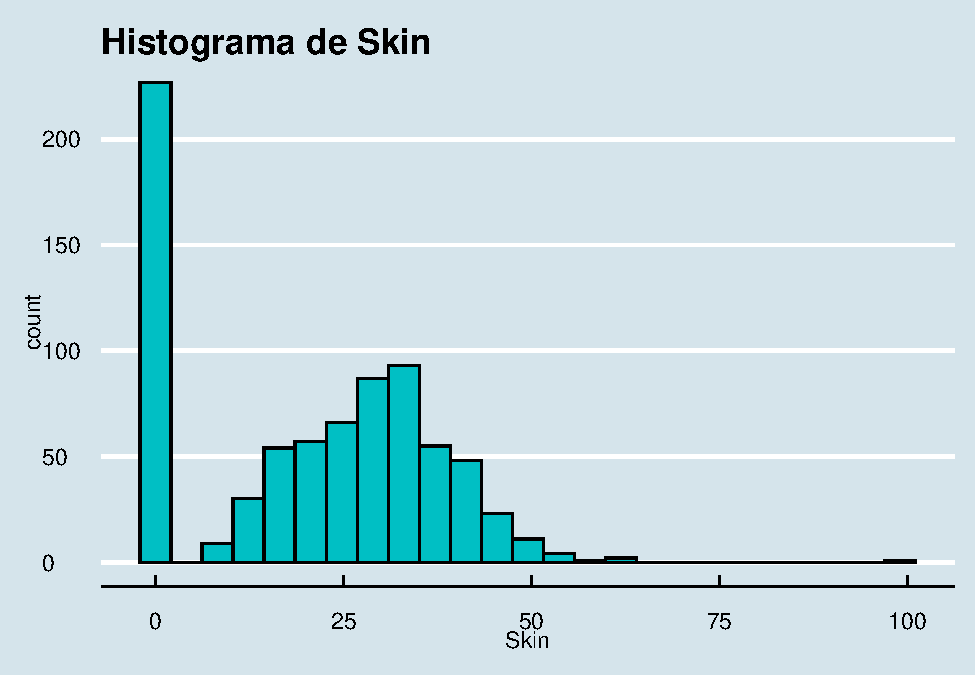
\includegraphics[width=0.5\linewidth]{pima-clasificacion_files/figure-latex/hist_skin-1} 

}

\caption{Histograma de Skin}\label{fig:hist_skin}
\end{figure}

Estudiando esos posibles valores perdidos vemos que hay 227 valores en
0, dado que Skin se refiere al grosor del pliegue cutáneo del tríceps no
tiene sentido que haya valores en 0, por lo que se tratan de valores
perdidos. Podemos ver que representan un 30\% de los valores, por lo que
eliminarlos nos dejaría con sólo el 70\% de los datos, por lo que no es
una opción. Por otro lado, en el caso de imputarlos de forma
generalizada (ya sea media o mediana), al ser tantos valores perdidos,
la imputación podría sesgar los datos. Lo más correcto sería usar algún
tipo de técnica que nos permita extraer información estimada de los
valores perdidos usando la información disponible del resto de variables
del dataset. Esto se podría conseguir con un KNN o una regresión lineal,
pero este no entra dentro del objetivo principal de este trabajo. Por
estas razones y dado que es una clasificación, se decide imputar
siguiendo la media de cada clase. Se elige la media dado que la
distribución es relativamente simétrica.

\begin{verbatim}
## [1] "Resumen antes de imputar:"
\end{verbatim}

\begin{verbatim}
##    Min. 1st Qu.  Median    Mean 3rd Qu.    Max.    NA's 
##    7.00   22.00   29.00   29.15   36.00   99.00     227
\end{verbatim}

\begin{verbatim}
## [1] "Media clase 'tested_negative': 27.2355"
\end{verbatim}

\begin{verbatim}
## [1] "Media clase 'tested_positive': 33"
\end{verbatim}

\begin{verbatim}
## [1] "Resumen después de imputar:"
\end{verbatim}

\begin{verbatim}
##    Min. 1st Qu.  Median    Mean 3rd Qu.    Max. 
##    7.00   25.00   28.00   29.25   33.00   99.00
\end{verbatim}

Estudiamos los cuantiles de la variable Skin y lo visualizamos con un
boxplot (Figura \ref{fig:box_skin}). Donde vemos que el 25\% de las
mujeres tienen un grosor del pliegue cutáneo del tríceps menor de 25 y
que solo un 25\% tiene un grosor del pliegue cutáneo del tríceps mayor
de 33. En el boxplot podemos apreciar como la mayoría de valores están
alredeor de la media, pero con algunos outliers en ambos extremos.

\begin{verbatim}
##   0%  25%  50%  75% 100% 
##    7   25   28   33   99
\end{verbatim}

\begin{figure}

{\centering 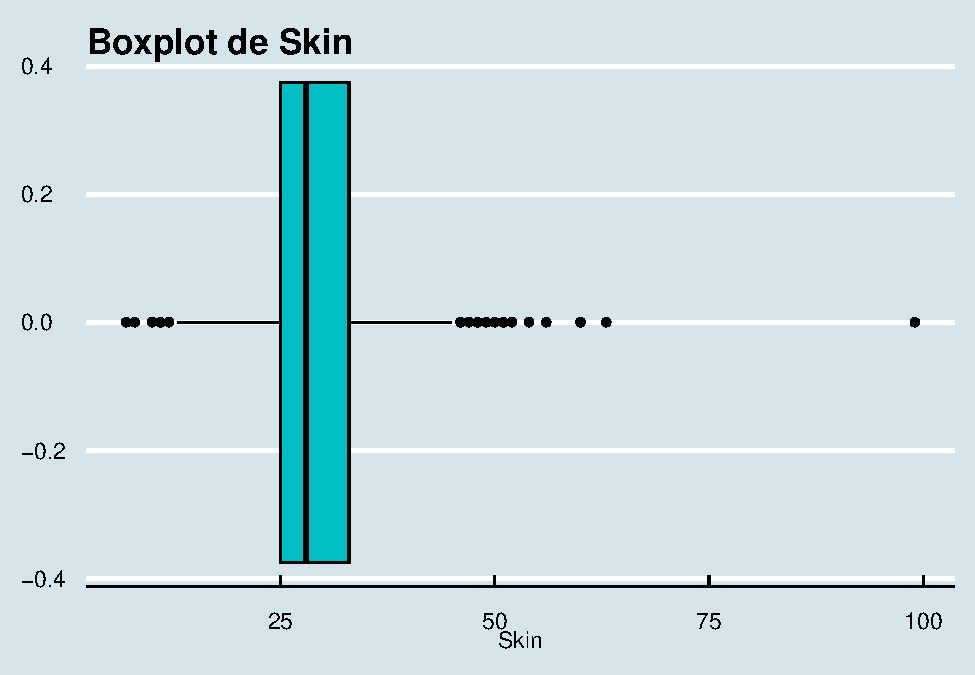
\includegraphics[width=0.5\linewidth]{pima-clasificacion_files/figure-latex/box_skin-1} 

}

\caption{Boxplot de Skin}\label{fig:box_skin}
\end{figure}

Estudiamos la forma de la variable Skin. Para ello miramos la media, sd,
skewness y kurtosis.

\begin{verbatim}
## [1] "Media: 29.247"
\end{verbatim}

\begin{verbatim}
## [1] "Desviación típica: 8.9239"
\end{verbatim}

Para estudiar la skewness y la kurtosis usaremos los tests de D'Agostino
y Anscombe respectivamente.

\begin{verbatim}
## [1] "Skewness: 0.7603"
\end{verbatim}

\begin{verbatim}
## 
##  D'Agostino skewness test
## 
## data:  pima$Skin
## skew = 0.76033, z = 7.77815, p-value = 7.36e-15
## alternative hypothesis: data have a skewness
\end{verbatim}

Dados que skewness \textgreater{} 0 la distribución está sesgada a la
derecha. Además el valor de p-value del test de D'agostino es menor que
0.05, por lo que podemos afirmar con seguridad que la distribución está
sesgada.

\begin{verbatim}
## [1] "Kurtosis: 7.8557"
\end{verbatim}

\begin{verbatim}
## 
##  Anscombe-Glynn kurtosis test
## 
## data:  pima$Skin
## kurt = 7.8557, z = 9.4860, p-value < 2.2e-16
## alternative hypothesis: kurtosis is not equal to 3
\end{verbatim}

Dado que kurtosis \textgreater{} 0 la distribución tiene colas pesadas.
Además el valor de p-value del test de Anscombe es menor de 0.05, por lo
que la ditribución tiene colas pesadas, y por lo tanto no es normal.
Podemos verlo mejor con un gráfico de densidad (Figura
\ref{fig:dens_skin}) donde observamos que la distribución presenta 2
picos, esto es consecuencia de la imputación de los valores perdidos.
Esto se puede visualizar mejor en el gráfico de densidad separado por
clase (Figura \ref{fig:dens_skin_class}). Por otro lado, realizamos el
test de Shapiro-Wilk para confirmar que la distribución no es normal y
lo visualizamos con un QQ-plot (Figura \ref{fig:qq_skin}).

\begin{verbatim}
## 
##  Shapiro-Wilk normality test
## 
## data:  pima$Skin
## W = 0.95267, p-value = 5.366e-15
\end{verbatim}

\begin{figure}

{\centering 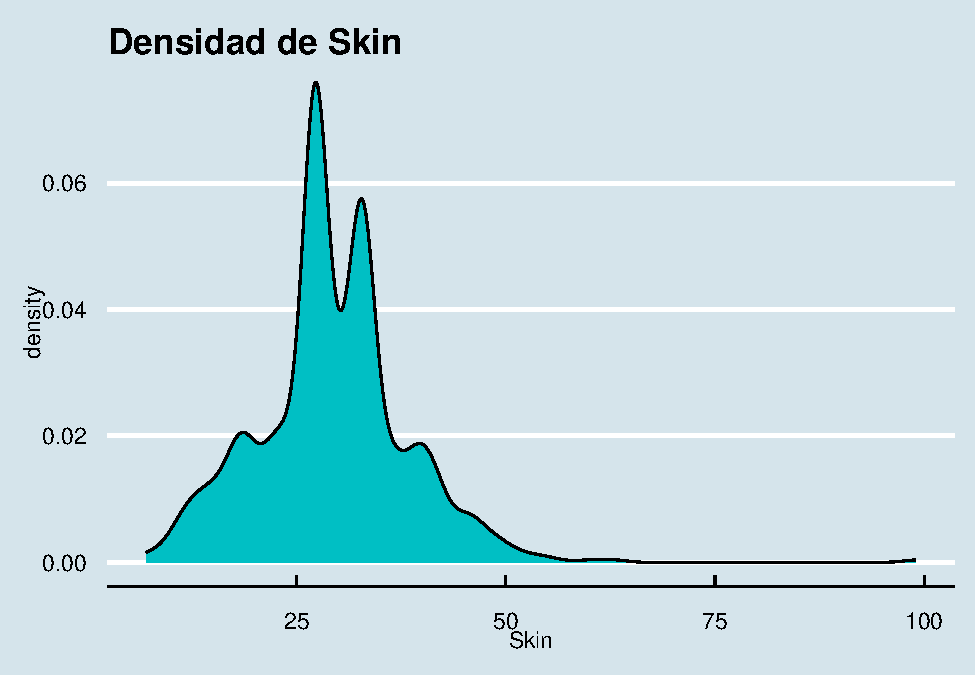
\includegraphics[width=0.5\linewidth]{pima-clasificacion_files/figure-latex/dens_skin-1} 

}

\caption{Densidad de Skin}\label{fig:dens_skin}
\end{figure}

\begin{figure}

{\centering 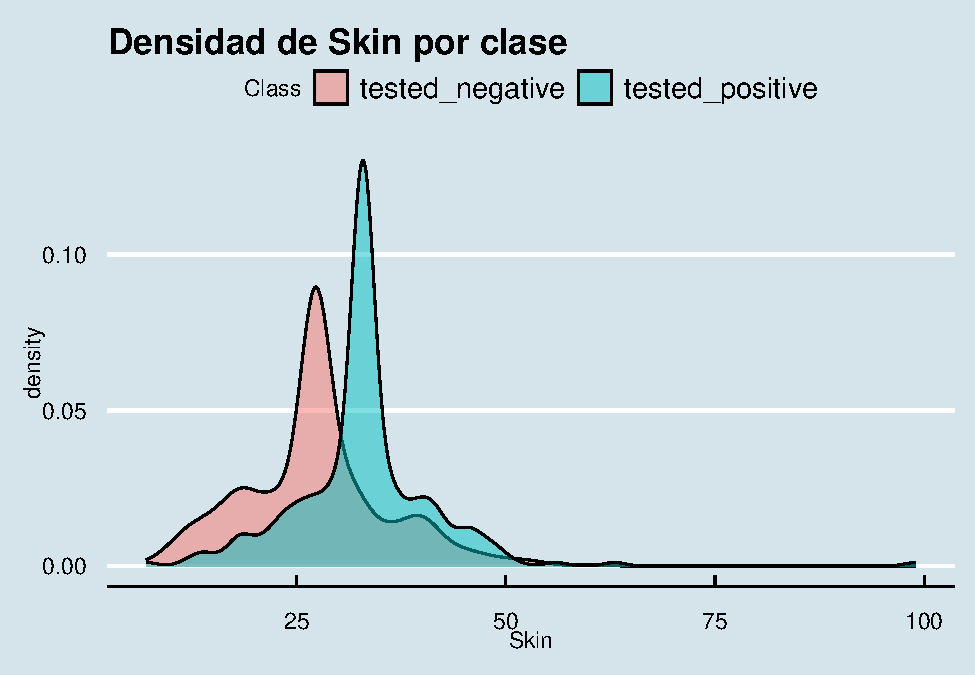
\includegraphics[width=0.5\linewidth]{pima-clasificacion_files/figure-latex/dens_skin_class-1} 

}

\caption{Densidad de Skin por clase}\label{fig:dens_skin_class}
\end{figure}

\begin{figure}

{\centering 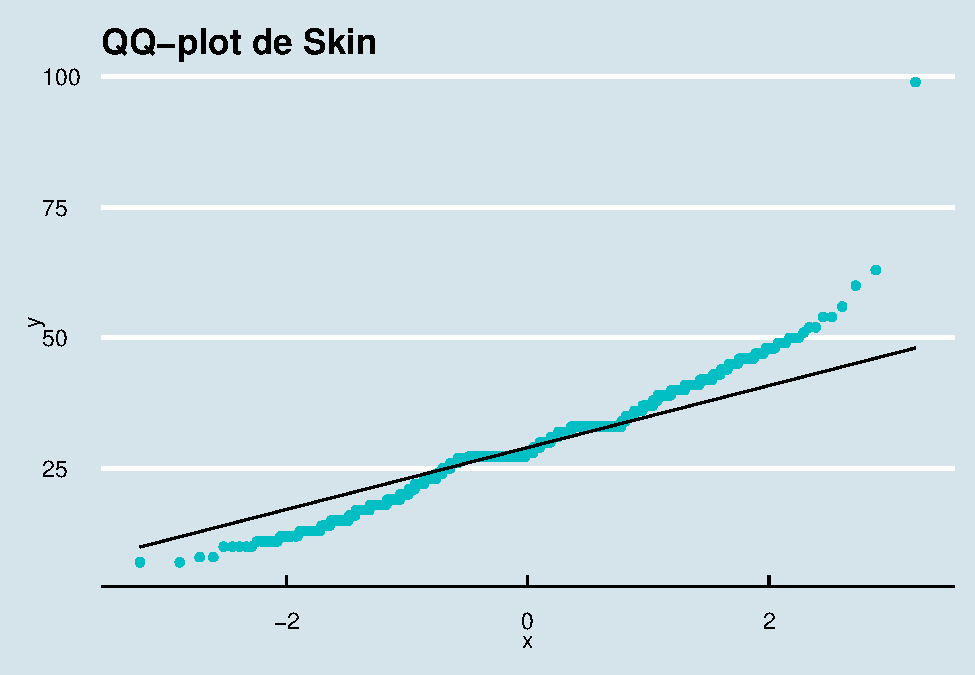
\includegraphics[width=0.5\linewidth]{pima-clasificacion_files/figure-latex/qq_skin-1} 

}

\caption{QQ-plot de Skin}\label{fig:qq_skin}
\end{figure}

\hypertarget{variable-insu}{%
\subsubsection{Variable `Insu'}\label{variable-insu}}

Continuamos estudiando ahora la variable Insu. Esta pertenece al rango
{[}0-846{]} y se refiere a la insulina sérica de 2 horas (mu U/ml). Para
más detalle vemos un histograma (Figura \ref{fig:hist_insu}). Se puede
observar que la mayoría de los valores se encuentran entre 0 y 200, con
un gran pico en 0 y con algunos valores a partir de 500 hasta 846. Esto
puede indicar que hay valores perdidos. Dado mi poco conocimiento sobre
el dataset y tras una búsqueda en internet, he encontrado que la
insulina sérica de 2 horas podría ser 0 en casos de ayuno por lo que no
podemos afirmar que los valores en 0 sean valores perdidos. Lo mismo con
los valores del rango superior, a partir de 800 se considera
hiperinsulinemia, por lo que tampoco podemos afirmar que sean valores
perdidos.

\begin{figure}

{\centering 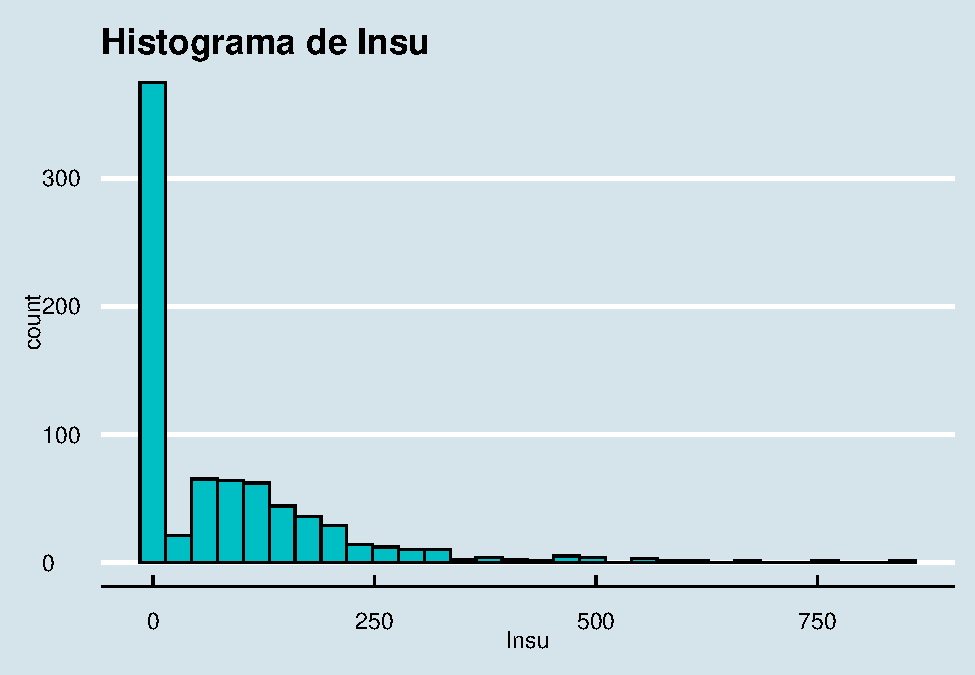
\includegraphics[width=0.5\linewidth]{pima-clasificacion_files/figure-latex/hist_insu-1} 

}

\caption{Histograma de Insu}\label{fig:hist_insu}
\end{figure}

Siguiendo con el análisis, vemos los cuantiles y lo visualizamos con un
boxplot (Figura \ref{fig:box_insu}). Observamos que el 25\% de las
mujeres tienen un nivel de insulina de 0, y que solo un 25\% tiene un
nivel de insulina mayor de 127. Podemos ver que parece ser una
distribución con valores atípicos en la parte superior, dejando una
larga cola.

\begin{verbatim}
##     0%    25%    50%    75%   100% 
##   0.00   0.00  30.50 127.25 846.00
\end{verbatim}

\begin{figure}

{\centering 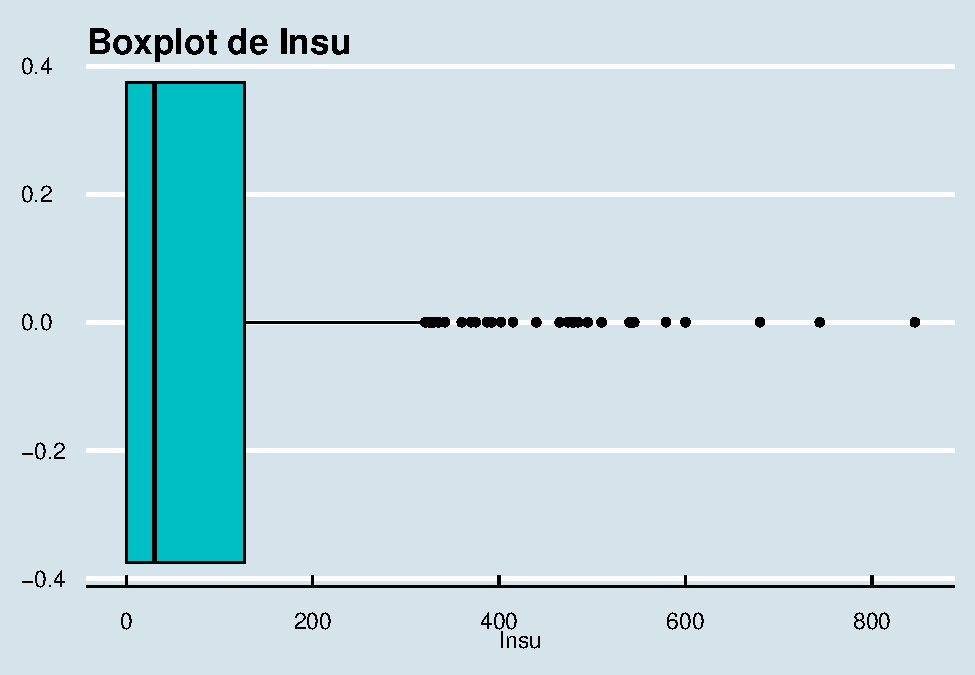
\includegraphics[width=0.5\linewidth]{pima-clasificacion_files/figure-latex/box_insu-1} 

}

\caption{Boxplot de Insu}\label{fig:box_insu}
\end{figure}

Estudiamos de seguido la forma de la variable Insu. Miramos la media,
sd, skewness y kurtosis.

\begin{verbatim}
## [1] "Media: 30"
\end{verbatim}

\begin{verbatim}
## [1] "Desviación típica: 115.244"
\end{verbatim}

Para estudiar la skewness y la kurtosis usaremos los tests de D'Agostino
y Anscombe respectivamente.

\begin{verbatim}
## [1] "Skewness: 2.2678"
\end{verbatim}

\begin{verbatim}
## 
##  D'Agostino skewness test
## 
## data:  pima$Insu
## skew = 2.2678, z = 16.3881, p-value < 2.2e-16
## alternative hypothesis: data have a skewness
\end{verbatim}

Dados que skewness \textgreater{} 0 la distribución está sesgada a la
derecha. Además el valor de p-value del test de D'agostino es menor que
0.05, por lo que podemos afirmar con seguridad que la distribución está
sesgada a la derecha.

\begin{verbatim}
## [1] "Kurtosis: 10.1596"
\end{verbatim}

\begin{verbatim}
## 
##  Anscombe-Glynn kurtosis test
## 
## data:  pima$Insu
## kurt = 10.160, z = 10.909, p-value < 2.2e-16
## alternative hypothesis: kurtosis is not equal to 3
\end{verbatim}

Dado que kurtosis \textgreater{} 0 la distribución tiene colas pesadas.
Además el valor de p-value del test de Anscombe es menor que 0.05, por
lo que podemos afirmar que la ditribución no es normal. Visualizamos la
forma con un gráfico de densidad (Figura \ref{fig:dens_insu}). Podemos
ver que la distribución es bastante asimétrica con una cola en la parte
superior muy pronunciada. Confirmamos la no normalidad con el test de
Shapiro-Wilk y visualizamos un QQ-plot (Figura \ref{fig:qq_insu}).

\begin{verbatim}
## 
##  Shapiro-Wilk normality test
## 
## data:  pima$Insu
## W = 0.72202, p-value < 2.2e-16
\end{verbatim}

\begin{figure}

{\centering 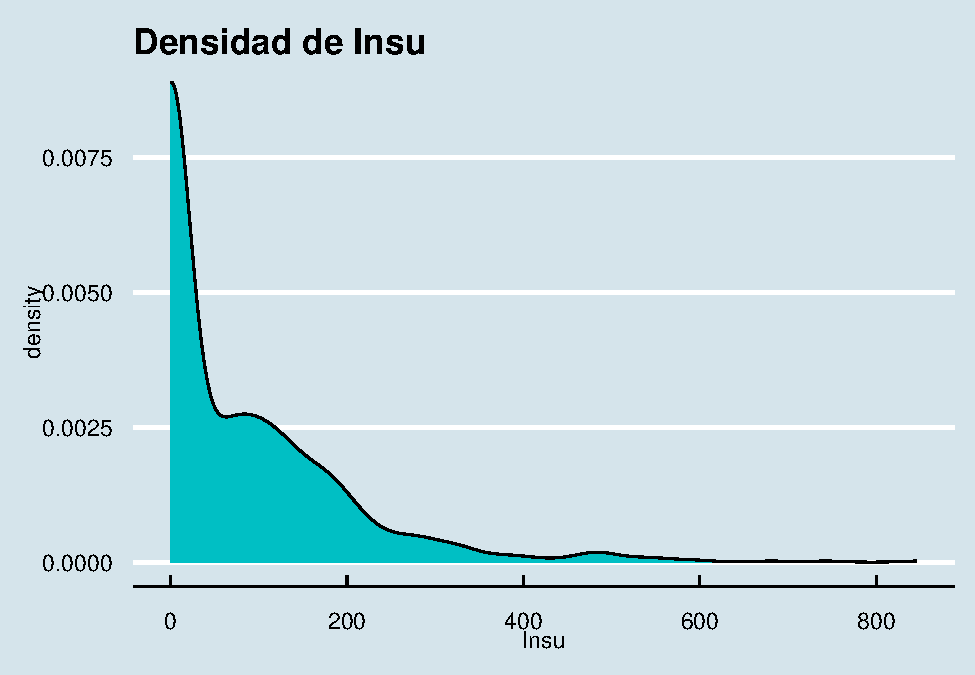
\includegraphics[width=0.5\linewidth]{pima-clasificacion_files/figure-latex/dens_insu-1} 

}

\caption{Densidad de Insu}\label{fig:dens_insu}
\end{figure}

\begin{figure}

{\centering 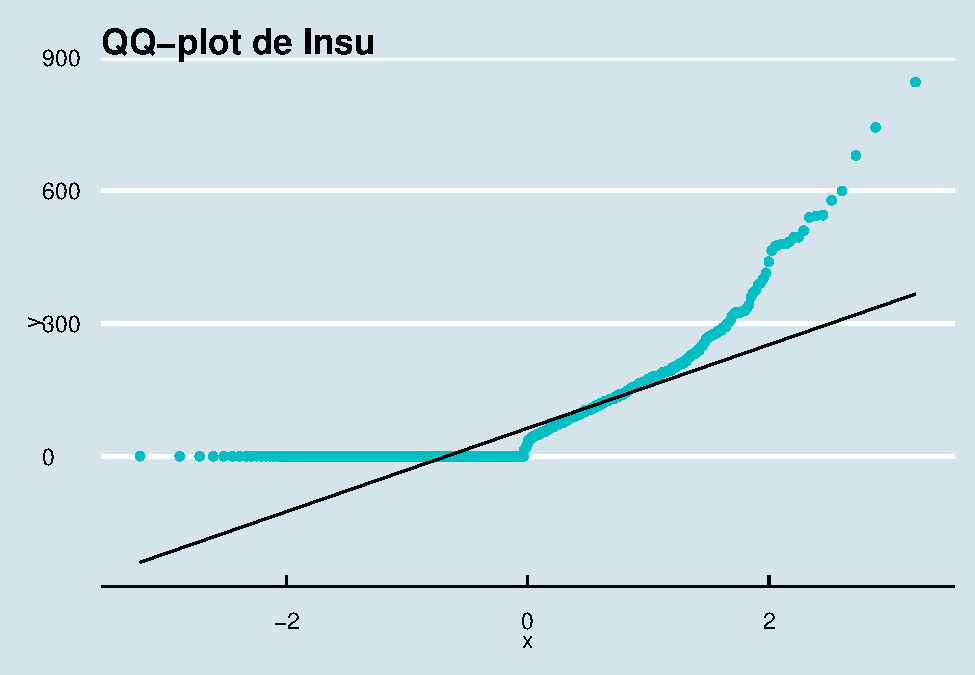
\includegraphics[width=0.5\linewidth]{pima-clasificacion_files/figure-latex/qq_insu-1} 

}

\caption{QQ-plot de Insu}\label{fig:qq_insu}
\end{figure}

\hypertarget{variable-mass}{%
\subsubsection{Variable `Mass'}\label{variable-mass}}

Ahora estudiamos la variable Mass. Esta pertece al rango {[}0-67.1{]} y
se refiere al índice de masa corporal (peso en kg/(altura en m)\^{}2).
Para más detalle vemos un histograma (Figura \ref{fig:hist_mass}). Se
puede observar que la mayoría de los valores se encuentran entre 20 y
45, con un pequeño pico en 0. Esto puede indicar que hay valores
perdidos.

\begin{figure}

{\centering 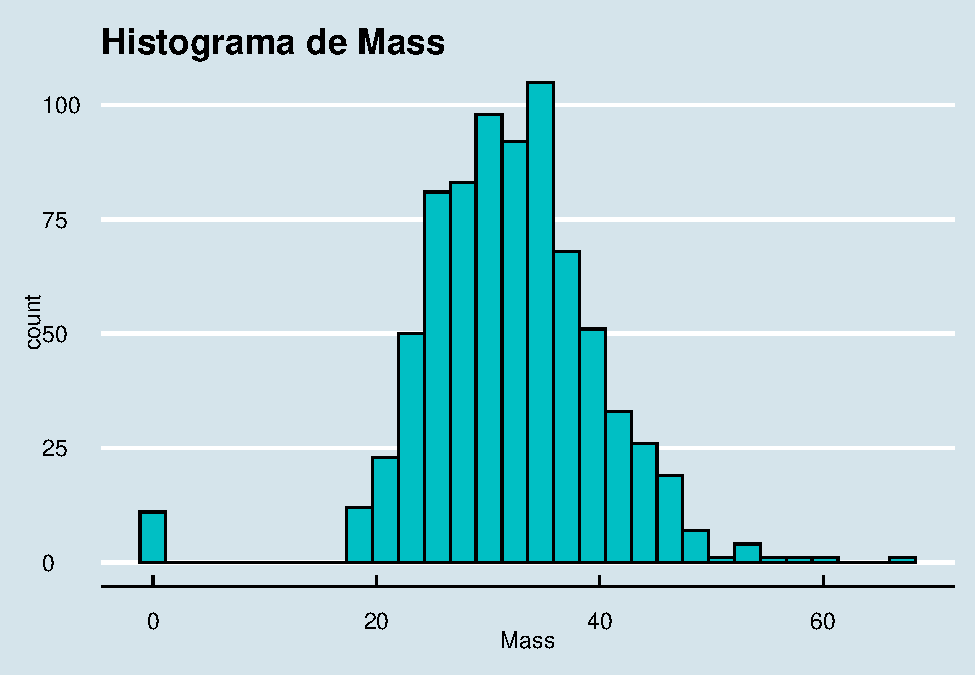
\includegraphics[width=0.5\linewidth]{pima-clasificacion_files/figure-latex/hist_mass-1} 

}

\caption{Histograma de Mass}\label{fig:hist_mass}
\end{figure}

Dada la naturaleza de la variable, no tiene sentido que haya valores en
0 dado que implicaría un peso de 0kg. Sustituimos estos valores por NA's
e imputamos los valores perdidos con la media ya que la variable es
bastante simétrica.

\begin{verbatim}
## [1] "Resumen antes de imputar:"
\end{verbatim}

\begin{verbatim}
##    Min. 1st Qu.  Median    Mean 3rd Qu.    Max.    NA's 
##   18.20   27.50   32.30   32.46   36.60   67.10      11
\end{verbatim}

\begin{verbatim}
## [1] "Resumen después de imputar:"
\end{verbatim}

\begin{verbatim}
##    Min. 1st Qu.  Median    Mean 3rd Qu.    Max. 
##   18.20   27.50   32.40   32.46   36.60   67.10
\end{verbatim}

Estudiamos los cuantiles y lo visualizamos con un boxplot (Figura
\ref{fig:box_mass}). Observamos que el 25\% de las mujeres tienen un
índice de masa corporal menor de 27.5 y que solo un 25\% tiene un índice
de masa corporal mayor de 36.6, teniendo una cola superior pronunciada.

\begin{verbatim}
##   0%  25%  50%  75% 100% 
## 18.2 27.5 32.4 36.6 67.1
\end{verbatim}

\begin{figure}

{\centering 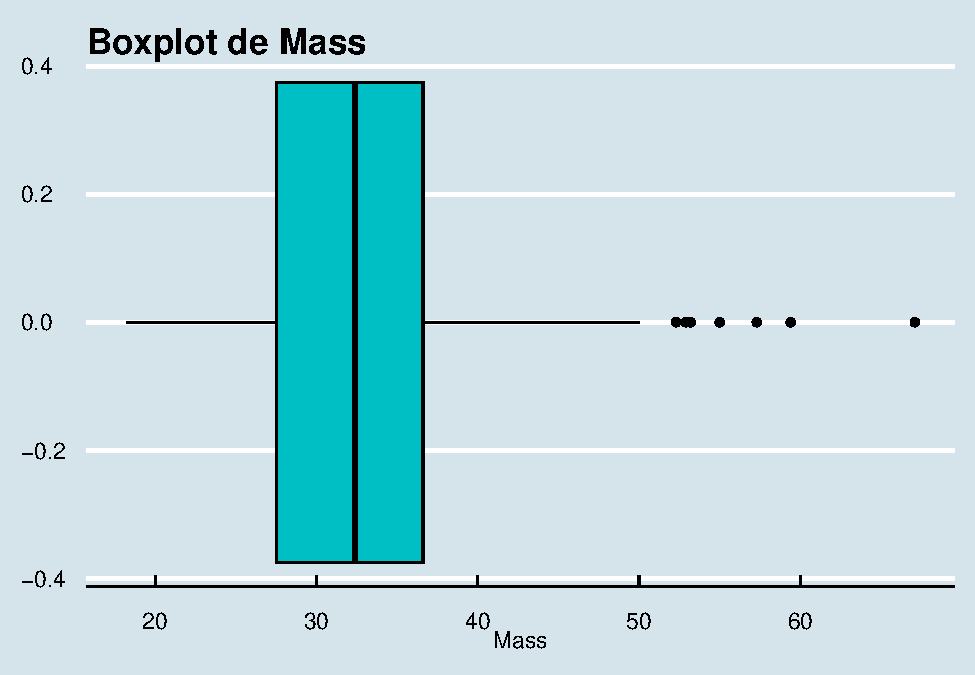
\includegraphics[width=0.5\linewidth]{pima-clasificacion_files/figure-latex/box_mass-1} 

}

\caption{Boxplot de Mass}\label{fig:box_mass}
\end{figure}

A continuación estudiamos la forma de la variable Mass. Miramos la
media, sd, skewness y kurtosis.

\begin{verbatim}
## [1] "Media: 32"
\end{verbatim}

\begin{verbatim}
## [1] "Desviación típica: 6.8752"
\end{verbatim}

Para estudiar la skewness y la kurtosis usaremos los tests de D'Agostino
y Anscombe respectivamente.

\begin{verbatim}
## [1] "Skewness: 0.5971"
\end{verbatim}

\begin{verbatim}
## 
##  D'Agostino skewness test
## 
## data:  pima$Mass
## skew = 0.59708, z = 6.33556, p-value = 2.365e-10
## alternative hypothesis: data have a skewness
\end{verbatim}

Dados que skewness \textgreater{} 0 la distribución está sesgada a la
derecha. Además el valor de p-value del test de D'agostino es menor que
0.05, por lo que podemos afirmar con seguridad que la distribución está
sesgada a la derecha.

\begin{verbatim}
## [1] "Kurtosis: 3.9057"
\end{verbatim}

\begin{verbatim}
## 
##  Anscombe-Glynn kurtosis test
## 
## data:  pima$Mass
## kurt = 3.9057, z = 3.7992, p-value = 0.0001452
## alternative hypothesis: kurtosis is not equal to 3
\end{verbatim}

Dado que kurtosis \textgreater{} 0 la distribución tiene colas pesadas.
Además el valor de p-value del test de Anscombe es menor que 0.05, por
lo que podemos afirmar que la ditribución no es normal. Visualizamos la
forma de la variable con un gráfico de densidad (Figura
\ref{fig:dens_mass}). Podemos ver que la distribución es algo simétrica
con una cola en la parte superior. Estudiamos la normalidad con el test
de Shapiro-Wilk y lo visualizamos con un QQ-plot (Figura
\ref{fig:qq_mass}).

\begin{verbatim}
## 
##  Shapiro-Wilk normality test
## 
## data:  pima$Mass
## W = 0.97946, p-value = 6.526e-09
\end{verbatim}

\begin{figure}

{\centering 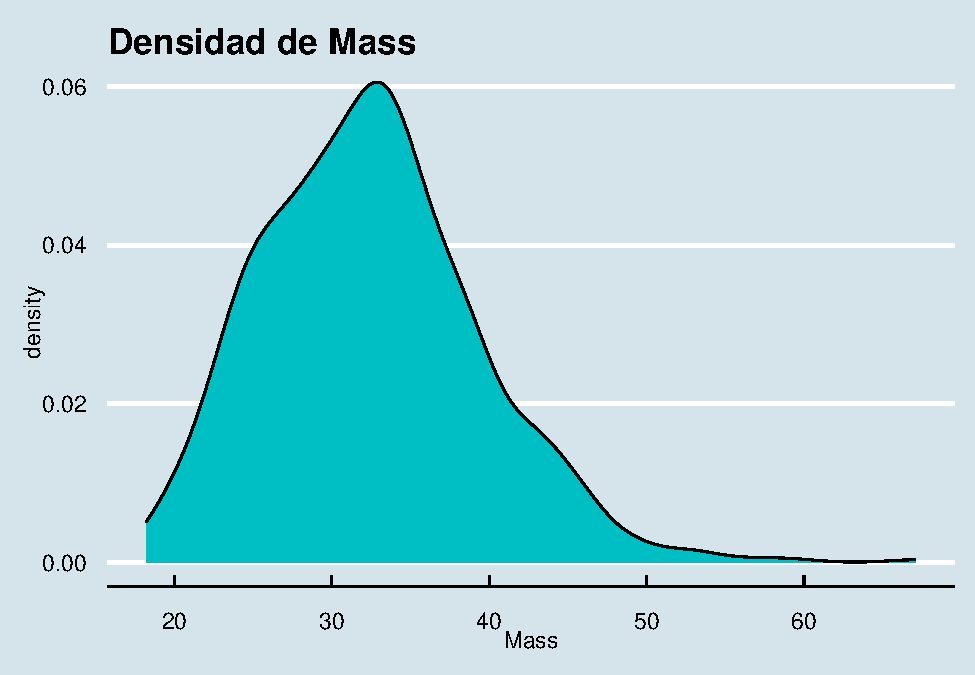
\includegraphics[width=0.5\linewidth]{pima-clasificacion_files/figure-latex/dens_mass-1} 

}

\caption{Densidad de Mass}\label{fig:dens_mass}
\end{figure}

\begin{figure}

{\centering 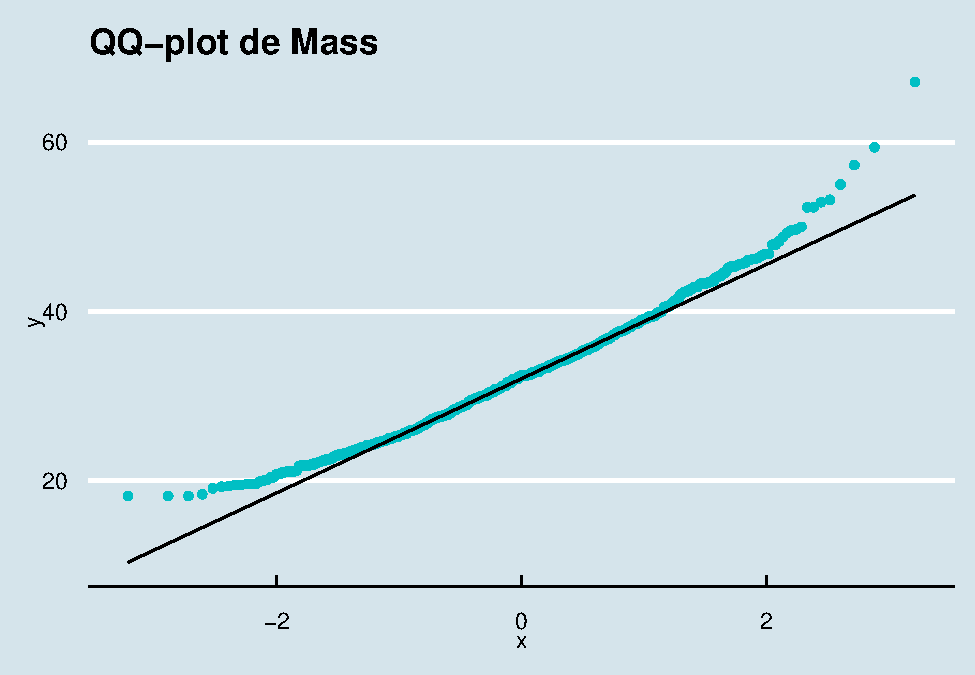
\includegraphics[width=0.5\linewidth]{pima-clasificacion_files/figure-latex/qq_mass-1} 

}

\caption{QQ-plot de Mass}\label{fig:qq_mass}
\end{figure}

\hypertarget{variable-pedi}{%
\subsubsection{Variable `Pedi'}\label{variable-pedi}}

Seguimos el análisis con la variable Pedi. Esta pertece al rango
{[}0.078-2.42{]} y se refiere a la función de pedigree de la diabetes.
Para más detalle vemos un histograma (Figura \ref{fig:hist_pedi}). Se
puede observar que la mayoría de los valores se encuentran entre 0 y
1.5, con una cola en la parte superior que alcanza hasta 2.5.

\begin{figure}

{\centering 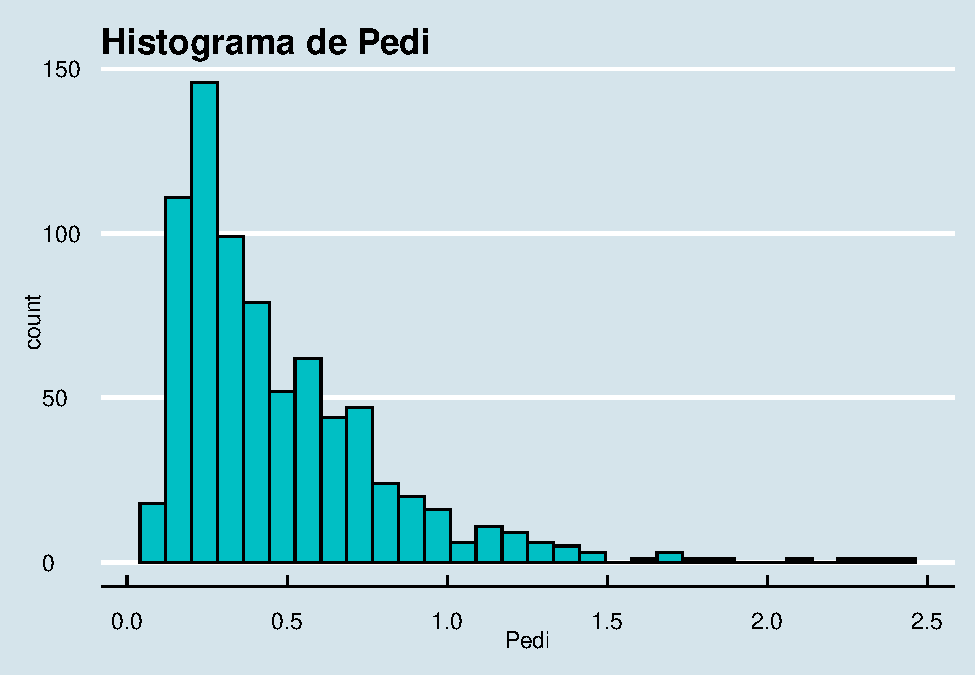
\includegraphics[width=0.5\linewidth]{pima-clasificacion_files/figure-latex/hist_pedi-1} 

}

\caption{Histograma de Pedi}\label{fig:hist_pedi}
\end{figure}

Estudiamos a continuación los cuantiles y lo visualizamos con un boxplot
(Figura \ref{fig:box_pedi}). Vemos que el 25\% de las mujeres tienen un
valor de Pedi menor de 0.24 y que solo un 25\% tiene un valor de Pedi
mayor de 0.63. Parece ser una distribución con valores atípicos en la
parte superior.

\begin{verbatim}
##      0%     25%     50%     75%    100% 
## 0.07800 0.24375 0.37250 0.62625 2.42000
\end{verbatim}

\begin{figure}

{\centering 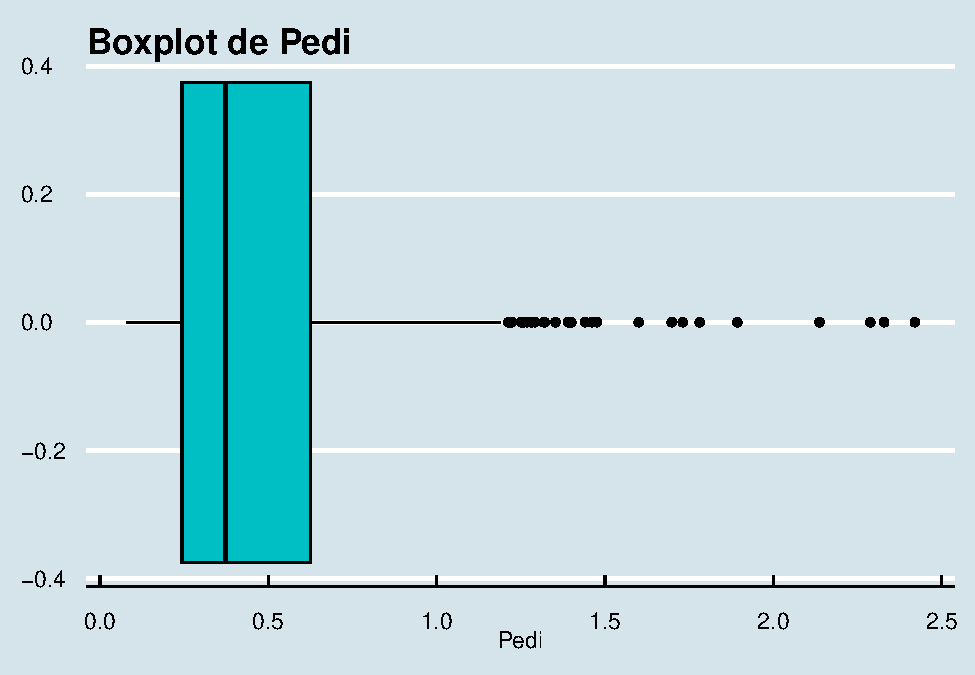
\includegraphics[width=0.5\linewidth]{pima-clasificacion_files/figure-latex/box_pedi-1} 

}

\caption{Boxplot de Pedi}\label{fig:box_pedi}
\end{figure}

Estudiamos a continuación la forma de la variable Pedi mirando la media,
sd, skewness y kurtosis.

\begin{verbatim}
## [1] "Media: 0"
\end{verbatim}

\begin{verbatim}
## [1] "Desviación típica: 0.3313"
\end{verbatim}

Para estudiar la skewness y la kurtosis usaremos los tests de D'Agostino
y Anscombe respectivamente.

\begin{verbatim}
## [1] "Skewness: 1.9162"
\end{verbatim}

\begin{verbatim}
## 
##  D'Agostino skewness test
## 
## data:  pima$Pedi
## skew = 1.9162, z = 14.9069, p-value < 2.2e-16
## alternative hypothesis: data have a skewness
\end{verbatim}

Dados que skewness \textgreater{} 0 la distribución está sesgada a la
derecha. Además el valor de p-value del test de D'agostino es menor que
0.05, por lo que podemos afirmar con seguridad que la distribución está
sesgada a la derecha.

\begin{verbatim}
## [1] "Kurtosis: 8.5508"
\end{verbatim}

\begin{verbatim}
## 
##  Anscombe-Glynn kurtosis test
## 
## data:  pima$Pedi
## kurt = 8.5508, z = 9.9811, p-value < 2.2e-16
## alternative hypothesis: kurtosis is not equal to 3
\end{verbatim}

Dado que kurtosis \textgreater{} 0 la distribución tiene colas pesadas.
Además el valor de p-value del test de Anscombe es menor que 0.05, por
lo que podemos afirmar que la ditribución no es normal. Visualizamos la
forma de la variable con un gráfico de densidad (Figura
\ref{fig:dens_pedi}). Podemos ver como la distribución es bastante
asimétrica con una cola en la parte superior. Confirmamos la no
normalidad con el test de Shapiro-Wilk y lo visualizamos con un QQ-plot
(Figura \ref{fig:qq_pedi}).

\begin{verbatim}
## 
##  Shapiro-Wilk normality test
## 
## data:  pima$Pedi
## W = 0.83652, p-value < 2.2e-16
\end{verbatim}

\begin{figure}

{\centering 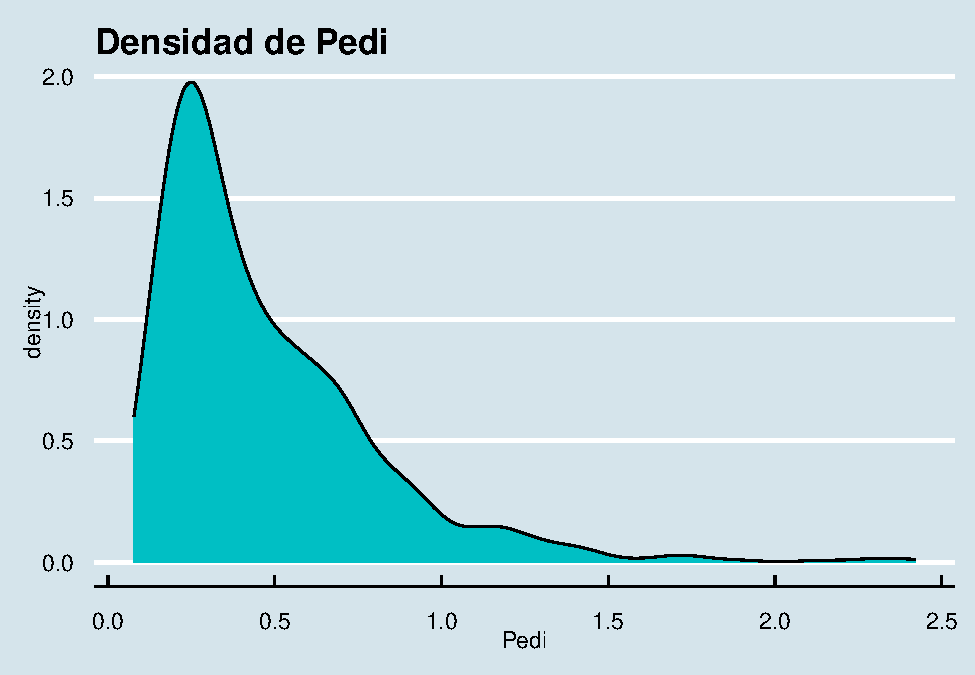
\includegraphics[width=0.5\linewidth]{pima-clasificacion_files/figure-latex/dens_pedi-1} 

}

\caption{Densidad de Pedi}\label{fig:dens_pedi}
\end{figure}

\begin{figure}

{\centering 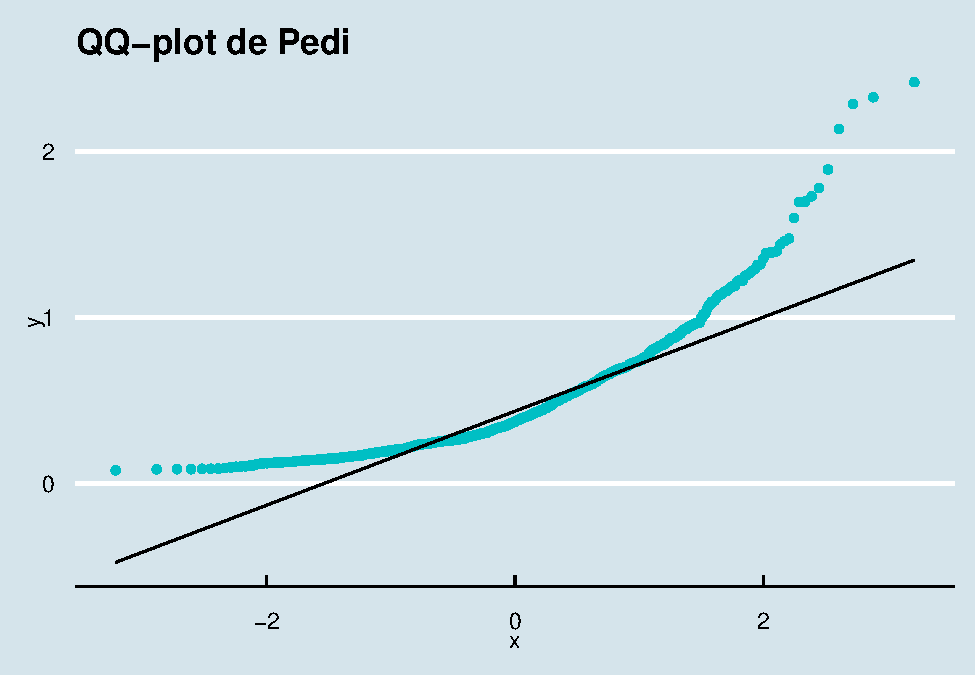
\includegraphics[width=0.5\linewidth]{pima-clasificacion_files/figure-latex/qq_pedi-1} 

}

\caption{QQ-plot de Pedi}\label{fig:qq_pedi}
\end{figure}

\hypertarget{variable-age}{%
\subsubsection{Variable `Age'}\label{variable-age}}

Estudiamos, por último, la variable Age. Esta pertece al rango
{[}21-81{]} y se refiere a la edad de la persona. Para más detalle vemos
un histograma (Figura \ref{fig:hist_age}). Se puede observar que la
mayoría de los valores se encuentran entre 20 y 40, con una cola en la
parte superior que alcanza hasta 80.

\begin{figure}

{\centering 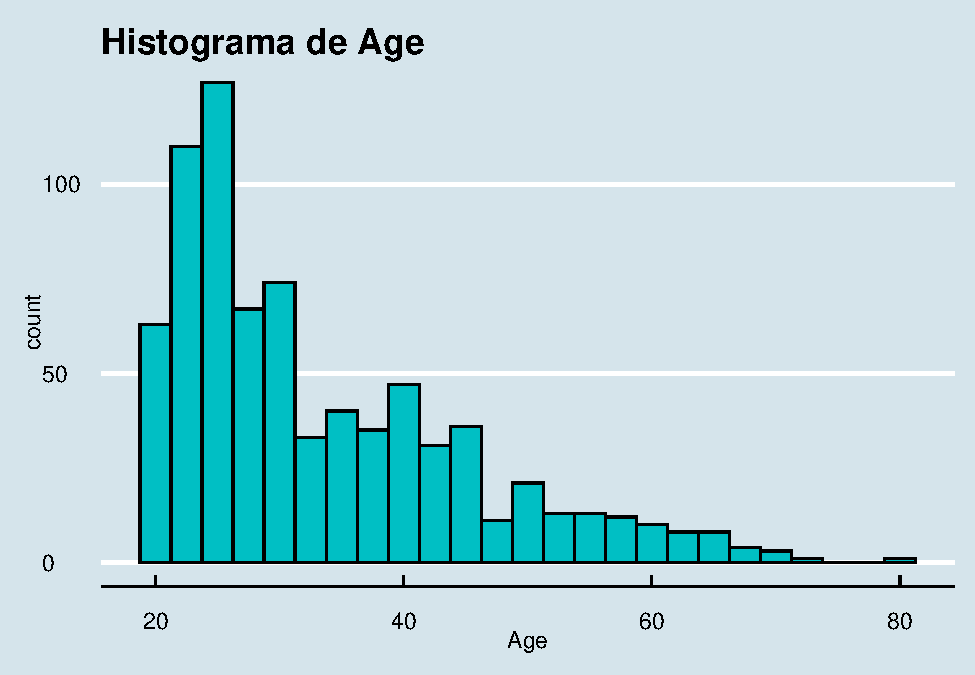
\includegraphics[width=0.5\linewidth]{pima-clasificacion_files/figure-latex/hist_age-1} 

}

\caption{Histograma de Age}\label{fig:hist_age}
\end{figure}

Estudiamos a continuación los cuantiles y lo visualizamos con un boxplot
(Figura \ref{fig:box_age}). Vemos que el 25\% de las mujeres tienen una
edad menor de 24 y que solo un 25\% tiene una edad mayor de 41. Parece
ser una distribución con valores atípicos en la parte superior.

\begin{verbatim}
##   0%  25%  50%  75% 100% 
##   21   24   29   41   81
\end{verbatim}

\begin{figure}

{\centering 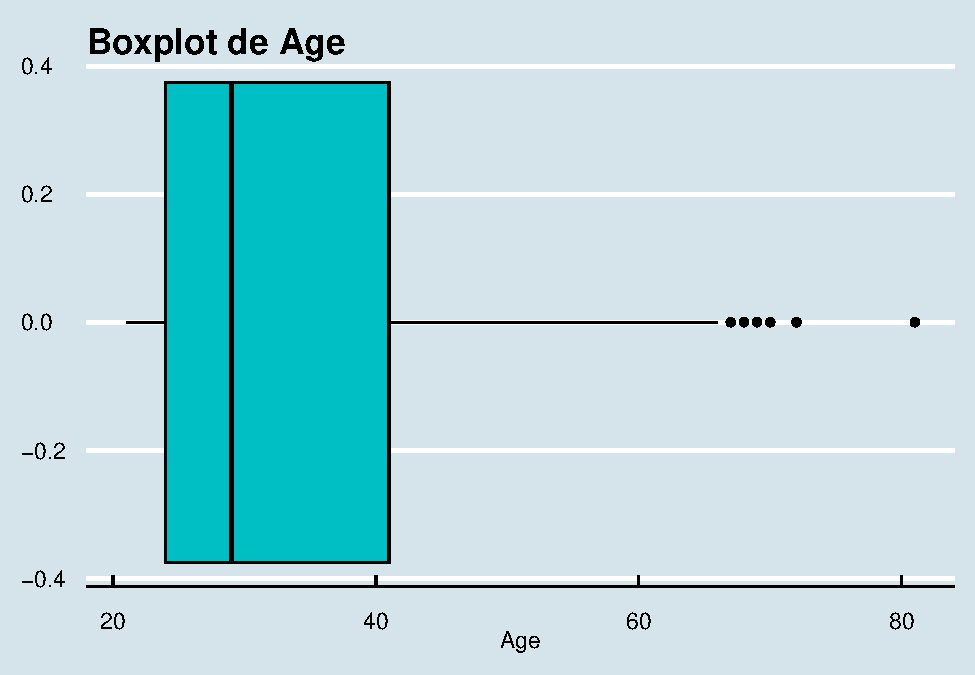
\includegraphics[width=0.5\linewidth]{pima-clasificacion_files/figure-latex/box_age-1} 

}

\caption{Boxplot de Age}\label{fig:box_age}
\end{figure}

Estudiamos la forma de la variable Age mirando la media, sd, skewness y
kurtosis.

\begin{verbatim}
## [1] "Media: 29"
\end{verbatim}

\begin{verbatim}
## [1] "Desviación típica: 11.7602"
\end{verbatim}

Para estudiar la skewness y la kurtosis usaremos los tests de D'Agostino
y Anscombe respectivamente.

\begin{verbatim}
## [1] "Skewness: 1.1274"
\end{verbatim}

\begin{verbatim}
## 
##  D'Agostino skewness test
## 
## data:  pima$Age
## skew = 1.1274, z = 10.5504, p-value < 2.2e-16
## alternative hypothesis: data have a skewness
\end{verbatim}

Dados que skewness \textgreater{} 0 la distribución está sesgada a la
derecha. Además el valor de p-value del test de D'agostino es menor que
0.05, por lo que podemos afirmar con seguridad que la distribución está
sesgada a la derecha.

\begin{verbatim}
## [1] "Kurtosis: 3.6312"
\end{verbatim}

\begin{verbatim}
## 
##  Anscombe-Glynn kurtosis test
## 
## data:  pima$Age
## kurt = 3.6312, z = 2.9267, p-value = 0.003425
## alternative hypothesis: kurtosis is not equal to 3
\end{verbatim}

Dado que kurtosis \textgreater{} 0 la distribución tiene colas pesadas.
Además el valor de p-value del test de Anscombe es menor que 0.05, por
lo que podemos afirmar que la ditribución no es normal. Visualizamos la
forma de la variable con un gráfico de densidad (Figura
\ref{fig:dens_age}). Podemos ver como la distribución es bastante
asimétrica con una cola en la parte superior. Confirmamos la no
normalidad con el test de Shapiro-Wilk y lo visualizamos con un QQ-plot
(Figura \ref{fig:qq_age}).

\begin{verbatim}
## 
##  Shapiro-Wilk normality test
## 
## data:  pima$Age
## W = 0.87477, p-value < 2.2e-16
\end{verbatim}

\begin{figure}

{\centering 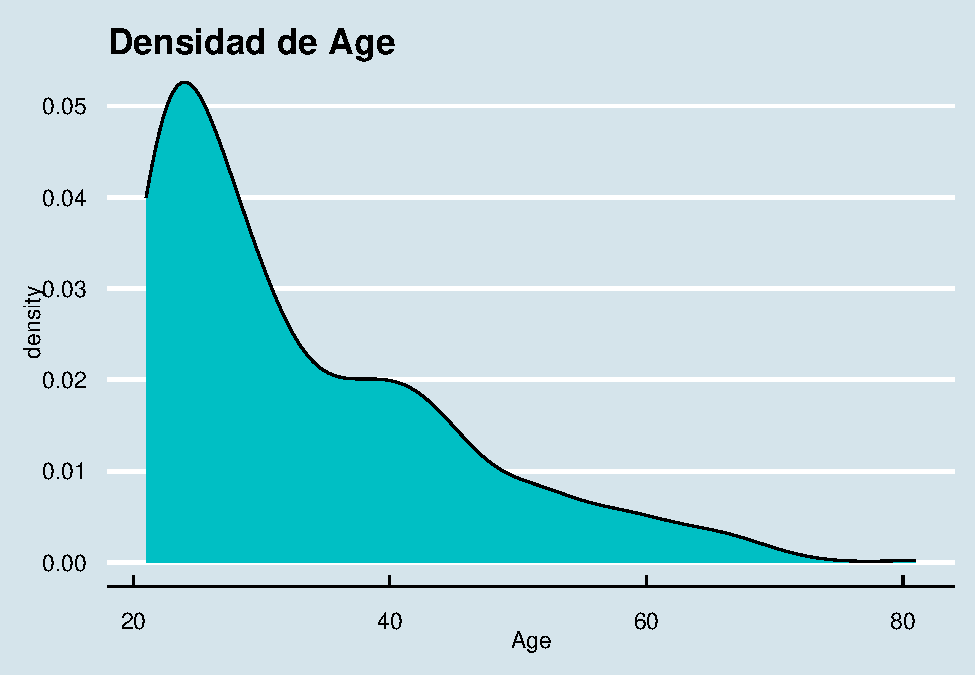
\includegraphics[width=0.5\linewidth]{pima-clasificacion_files/figure-latex/dens_age-1} 

}

\caption{Densidad de Age}\label{fig:dens_age}
\end{figure}

\begin{figure}

{\centering 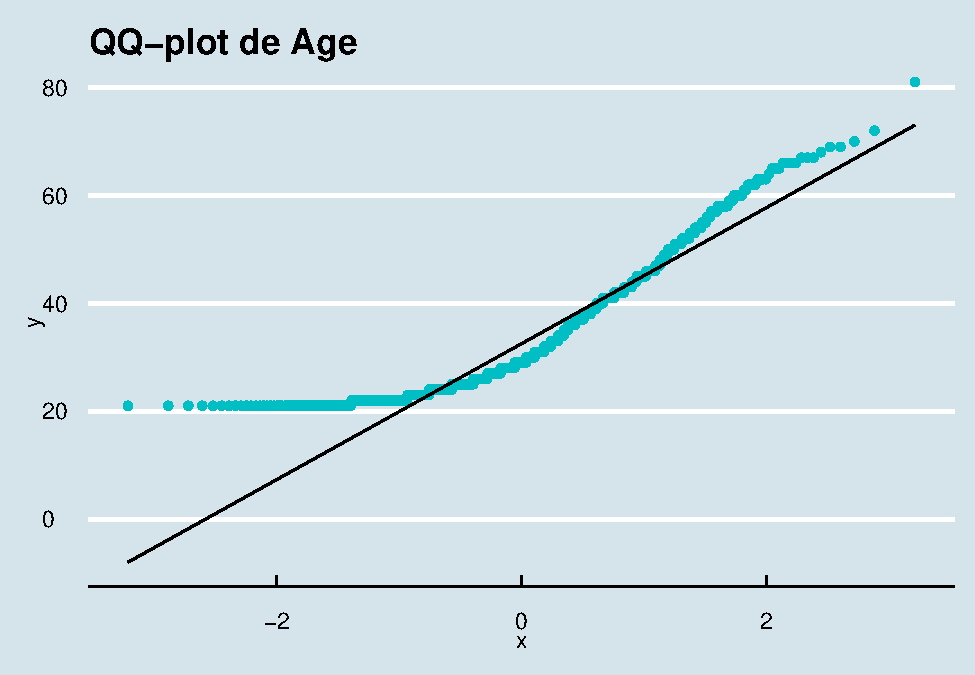
\includegraphics[width=0.5\linewidth]{pima-clasificacion_files/figure-latex/qq_age-1} 

}

\caption{QQ-plot de Age}\label{fig:qq_age}
\end{figure}

\hypertarget{anuxe1lisis-bivariable}{%
\subsection{Análisis bivariable}\label{anuxe1lisis-bivariable}}

Tras el análisis de cada variable por separado, haremos un análisis
bivariable, donde veremos la relación entre las variables.

\hypertarget{correlaciuxf3n}{%
\subsubsection{Correlación}\label{correlaciuxf3n}}

Para ver la correlación entre las variables numéricas usaremos el método
de Spearman pues las variables no siguen una distribución normal (ver
Figura \ref{fig:corr}).

\begin{figure}

{\centering 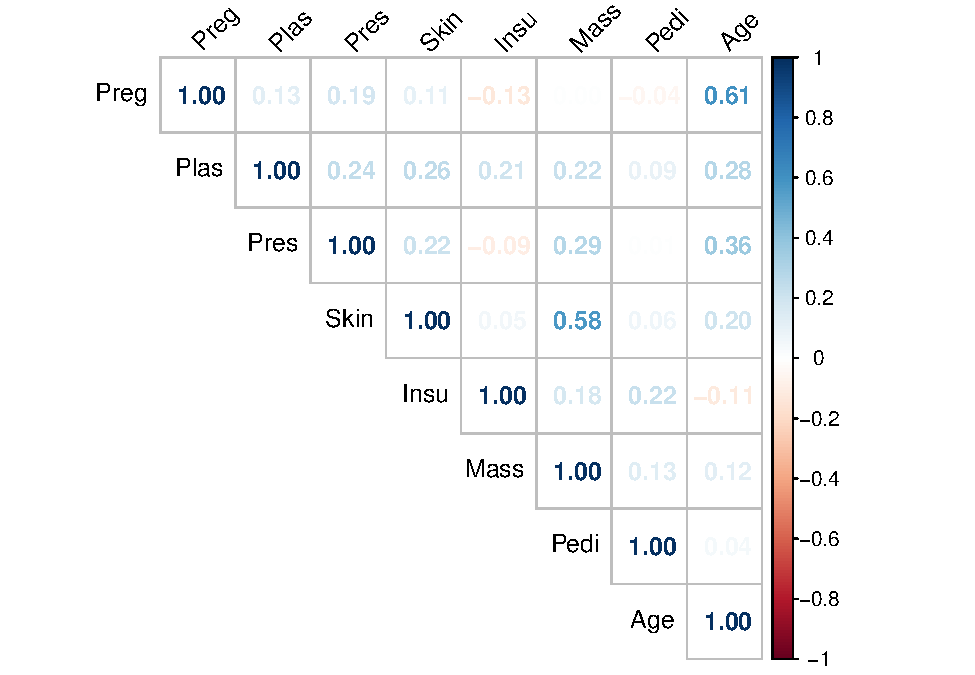
\includegraphics[width=0.75\linewidth]{pima-clasificacion_files/figure-latex/corr-1} 

}

\caption{Correlación entre variables numéricas}\label{fig:corr}
\end{figure}

Vemos que las variables que más correlación tienen, aunque no muy
significativa, son Skin con Mass y Age con Preg. Lo cual tiene sentido
pues la edad de la persona está relacionada con el número de embarazos
ya que a mayor número de embarazos, necesariamente, mayor edad. Además,
la variable Skin está relacionada con Mass pues a mayor masa corporal,
mayor grosor de la piel.

\hypertarget{scatterplots}{%
\subsubsection{Scatterplots}\label{scatterplots}}

Para ver mejor las relaciones de las variables con mayor correlación
vamos a hacer un scatterplot de cada una de estas parejas (ver Figura
\ref{fig:scatter}). Vemos que para la pareja Skin y Mass hay una
relación lineal positiva entre ambas variables y los puntos se
aconglomeran pero con una clara tendencia. Por otro lado, para Age y
Preg vemos que hay una relación lineal positiva entre ambas variables
pero los puntos se dispersan significativamente de la recta.

\begin{figure}

{\centering 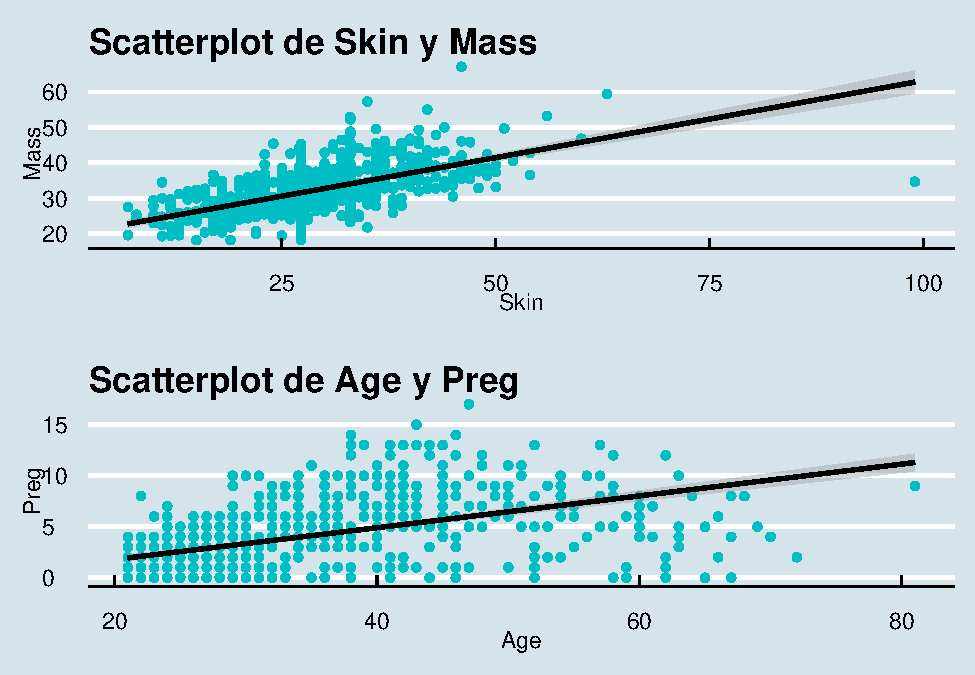
\includegraphics[width=0.5\linewidth]{pima-clasificacion_files/figure-latex/scatter-1} 

}

\caption{Scatterplots de las variables con mayor correlación}\label{fig:scatter}
\end{figure}

\hypertarget{relaciuxf3n-con-la-variable-class}{%
\subsubsection{Relación con la variable
Class}\label{relaciuxf3n-con-la-variable-class}}

Ahora vamos a ver la relación entre las variables numéricas y la
variable Class. Para ello hacemos un boxplot de cada variable numérica
con respecto a la variable Class (Figura \ref{fig:multi_boxplot}). Vemos
que todas las variables, en general, indican que las mujeres con
diabetes tienen valores más altos que las mujeres sin diabetes.
Principalmente son interesantes las variables Plas y la variable Skin
cuyos percentiles 25 en la clase positiva, son mayores que los
percentiles 75 de la clase negativa.

\begin{figure}

{\centering 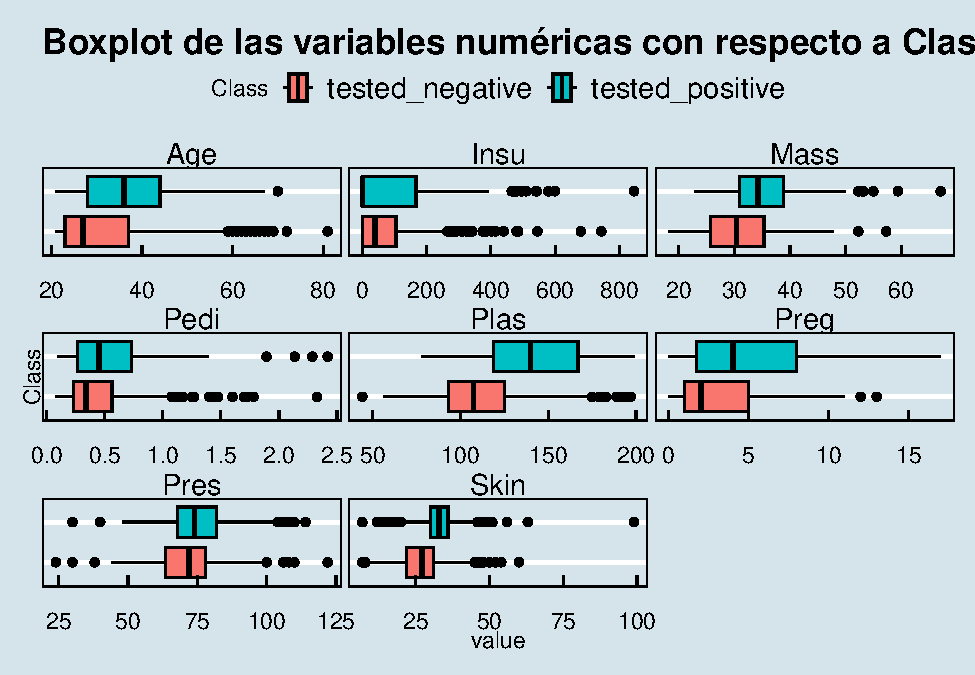
\includegraphics[width=1\linewidth]{pima-clasificacion_files/figure-latex/multi_boxplot-1} 

}

\caption{Boxplot de las variables numéricas con respecto a Class}\label{fig:multi_boxplot}
\end{figure}

\hypertarget{modelos-de-clasificaciuxf3n}{%
\section{Modelos de clasificación}\label{modelos-de-clasificaciuxf3n}}

\hypertarget{metologuxeda-de-trabajo}{%
\subsection{Metología de trabajo}\label{metologuxeda-de-trabajo}}

Para la realización de los modelos de clasificación, se pide usar las
técnicas de K-NN, LDA y QDA. Para ello, primeramente se preparán los
datos y se separa el dataset en train y test. Posteriormente, se entrena
el modelo con los datos de train y se evalúa con los datos de test.
Finalmente, se evalúa el modelo con los datos de test y se calcula la
matriz de confusión y el accuracy.

\hypertarget{preparaciuxf3n-de-los-datos}{%
\subsection{Preparación de los
datos}\label{preparaciuxf3n-de-los-datos}}

Para poder utilizar los modelos de clasificación, debemos preparar los
datos. Para ello, primero separamos la variable Class del resto de
variables, normalizamos los datos y separmos el conjunto de datos en
train y test (80\% y 20\% respectivamente).

\begin{Shaded}
\begin{Highlighting}[]
\FunctionTok{set.seed}\NormalTok{(}\DecValTok{123}\NormalTok{)}

\NormalTok{pima\_data }\OtherTok{\textless{}{-}}\NormalTok{ pima }\SpecialCharTok{\%\textgreater{}\%}\NormalTok{ dplyr}\SpecialCharTok{::}\FunctionTok{select}\NormalTok{(}\SpecialCharTok{{-}}\NormalTok{Class)}

\NormalTok{pObj }\OtherTok{\textless{}{-}} \FunctionTok{preProcess}\NormalTok{(pima\_data, }\AttributeTok{method=}\FunctionTok{c}\NormalTok{(}\StringTok{\textquotesingle{}range\textquotesingle{}}\NormalTok{))}
\NormalTok{pima\_scaled }\OtherTok{\textless{}{-}} \FunctionTok{predict}\NormalTok{(pObj, pima\_data)}

\NormalTok{test\_size }\OtherTok{\textless{}{-}} \FloatTok{0.2}
\NormalTok{train\_size }\OtherTok{\textless{}{-}} \DecValTok{1} \SpecialCharTok{{-}}\NormalTok{ test\_size}

\NormalTok{train\_indices }\OtherTok{\textless{}{-}} \FunctionTok{createDataPartition}\NormalTok{(pima}\SpecialCharTok{$}\NormalTok{Class, }\AttributeTok{p=}\NormalTok{train\_size, }\AttributeTok{list=}\ConstantTok{FALSE}\NormalTok{)}
\NormalTok{train }\OtherTok{\textless{}{-}}\NormalTok{ pima\_scaled[train\_indices, ]}
\NormalTok{test }\OtherTok{\textless{}{-}}\NormalTok{ pima\_scaled[}\SpecialCharTok{{-}}\NormalTok{train\_indices, ]}
\NormalTok{train\_lbls }\OtherTok{\textless{}{-}}\NormalTok{ pima[train\_indices, ]}\SpecialCharTok{$}\NormalTok{Class}
\NormalTok{test\_lbls }\OtherTok{\textless{}{-}}\NormalTok{ pima[}\SpecialCharTok{{-}}\NormalTok{train\_indices, ]}\SpecialCharTok{$}\NormalTok{Class}
\end{Highlighting}
\end{Shaded}

\hypertarget{k-nn-k-nearest-neighbors}{%
\subsection{K-NN (K-Nearest Neighbors)}\label{k-nn-k-nearest-neighbors}}

K-NN se basa en la idea de que los puntos de datos con etiquetas
similares se encuentran cerca unos de otros en el espacio. Por lo tanto
elegir un correcto valor de K es crucial. Para ello, se usa la función
`train' de la librería `caret' para encontrar el valor de K óptimo.
Usaremos la función \texttt{trainControl()} para realizar validación
cruzada repetida 10 veces y con 5 repeticiones.

\begin{verbatim}
## [1] "K óptimo: 27"
\end{verbatim}

\begin{figure}

{\centering 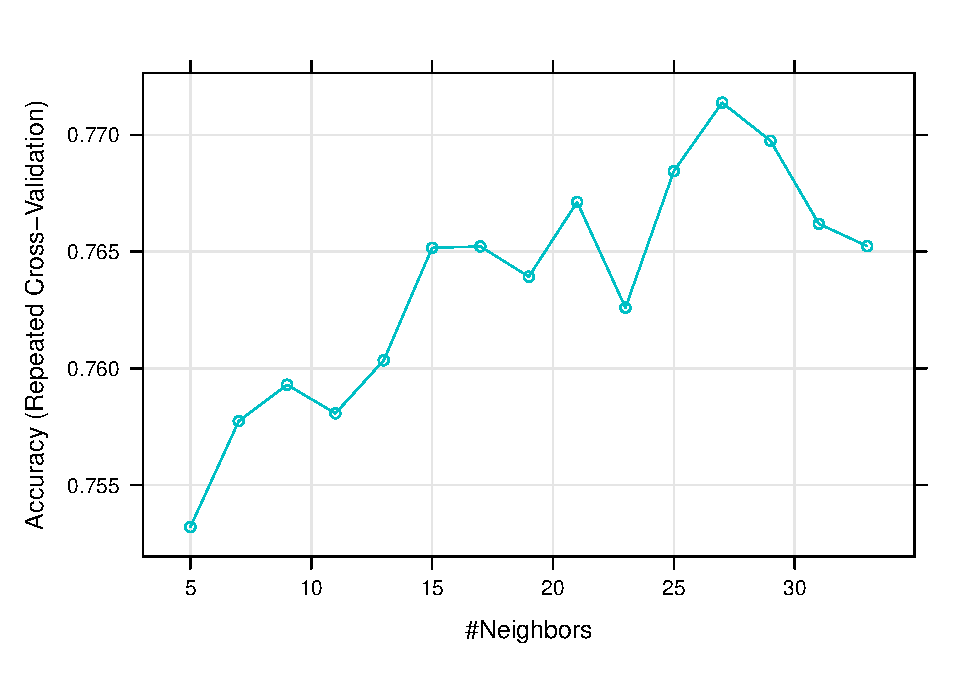
\includegraphics[width=0.5\linewidth]{pima-clasificacion_files/figure-latex/k_plot-1} 

}

\caption{Accuracy en función de K}\label{fig:k_plot}
\end{figure}

Vemos que el valor óptimo es 27 (Figura \ref{fig:k_plot}). Ahora,
evaluamos el modelo con el conjunto de test y calculamos la matriz de
confusión y el accuracy. Podemos ver que el accuracy es cercano al 80\%
pero nos interesa más el recall, que es la capacidad del modelo de
encontrar todos los casos positivos. En este caso, el recall es de 0.58
relativamente menor que el accuracy general.

\begin{verbatim}
## Confusion Matrix and Statistics
## 
##                  Reference
## Prediction        tested_negative tested_positive
##   tested_negative              90              22
##   tested_positive              10              31
##                                           
##                Accuracy : 0.7908          
##                  95% CI : (0.7178, 0.8523)
##     No Information Rate : 0.6536          
##     P-Value [Acc > NIR] : 0.0001499       
##                                           
##                   Kappa : 0.5122          
##                                           
##  Mcnemar's Test P-Value : 0.0518299       
##                                           
##               Precision : 0.7561          
##                  Recall : 0.5849          
##                      F1 : 0.6596          
##              Prevalence : 0.3464          
##          Detection Rate : 0.2026          
##    Detection Prevalence : 0.2680          
##       Balanced Accuracy : 0.7425          
##                                           
##        'Positive' Class : tested_positive 
## 
\end{verbatim}

\hypertarget{fold-cross-validation}{%
\subsubsection{10 - fold cross validation}\label{fold-cross-validation}}

Ahora, vamos a realizar validación cruzada de 10 folds para ver si el
accuracy es similar al obtenido anteriormente. El dataset ya viene con
las particiones preparadas así que las cargamos en memoria y realizamos
el entrenamiento y evaluación del modelo. Los resultados se pueden ver
en la Figura \ref{fig:10f_knn} y estos son similares a los obtenidos
anteriormente.

\begin{figure}

{\centering 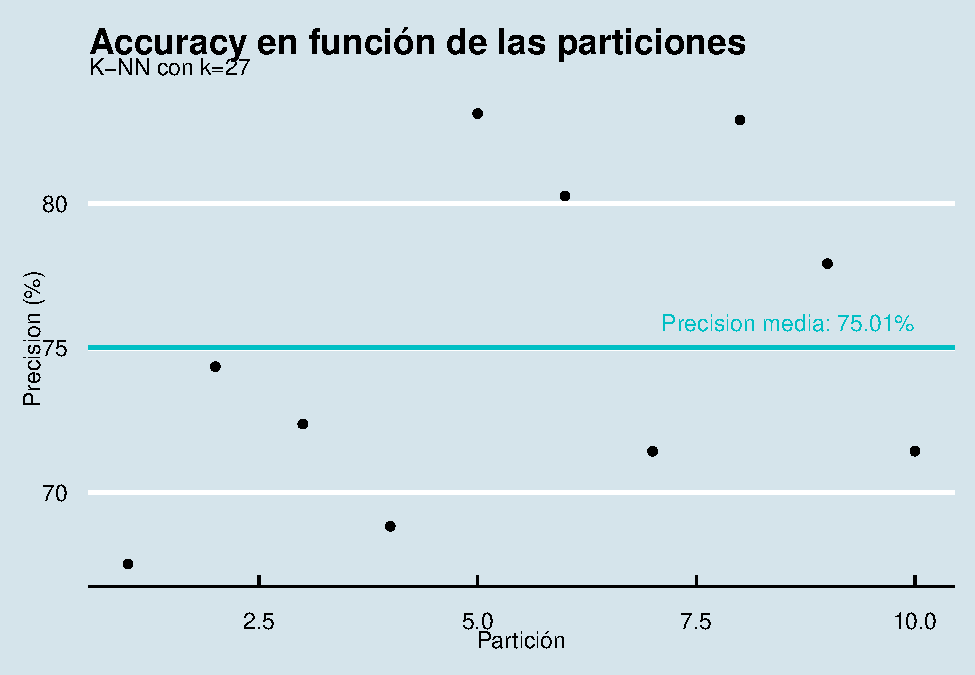
\includegraphics[width=0.5\linewidth]{pima-clasificacion_files/figure-latex/10f_knn-1} 

}

\caption{Accuracy en función de las particiones para KNN}\label{fig:10f_knn}
\end{figure}

\hypertarget{discriminant-analysis}{%
\subsection{Discriminant Analysis}\label{discriminant-analysis}}

En este apartado usaremos LDA (Linear Discriminant Analysis) y su
versión cuadrática QDA (Quadratic Discriminant Analysis). Para ello,
usaremos la librería `MASS' y su funciones `lda()' y 'qda(). Ambas que
las variables siguen una distribución normal, LDA que las matrices de
covarianza son iguales para todas las clases y QDA permite que cada
variable tenga su matriz de covarianza. Por lo tanto, debemos
asegurarnos de que las variables estén normalizadas para cada clase.
Visualizamos la distribución de cada variable para cada clase (Figura
\ref{fig:multi_density}). Vemos que hay que normalizar todas las
variables por su media y desviación típica. Los resultados podemos
verlos en la Figura \ref{fig:multi_norm_density}.

\begin{figure}

{\centering 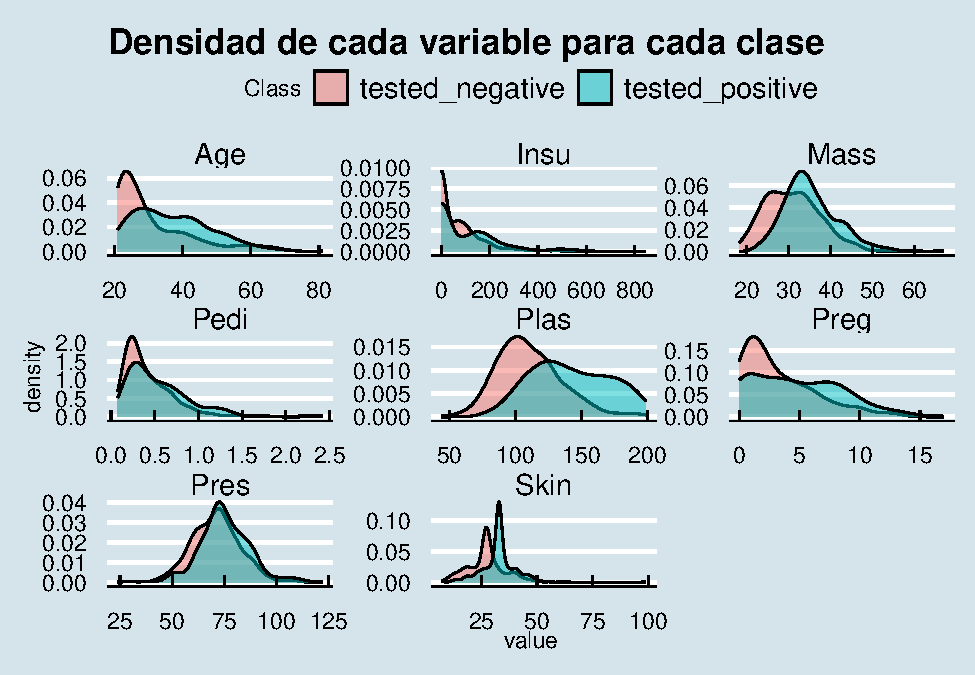
\includegraphics[width=0.75\linewidth]{pima-clasificacion_files/figure-latex/multi_density-1} 

}

\caption{Distribución de cada variable para cada clase}\label{fig:multi_density}
\end{figure}

\begin{verbatim}
## [1] "Datos normalizados:"
\end{verbatim}

\begin{verbatim}
##       Preg              Plas              Pres              Skin        
##  Min.   :-1.3006   Min.   :-2.6989   Min.   :-3.9339   Min.   :-3.0747  
##  1st Qu.:-0.7616   1st Qu.:-0.7165   1st Qu.:-0.5983   1st Qu.:-0.4973  
##  Median :-0.2314   Median :-0.1096   Median :-0.0784   Median : 0.0000  
##  Mean   : 0.0000   Mean   : 0.0000   Mean   : 0.0000   Mean   : 0.0000  
##  3rd Qu.: 0.5705   3rd Qu.: 0.6591   3rd Qu.: 0.5921   3rd Qu.: 0.3548  
##  Max.   : 3.2434   Max.   : 3.4911   Max.   : 4.2800   Max.   : 7.8050  
##       Insu              Mass              Pedi              Age         
##  Min.   :-0.7235   Min.   :-1.9506   Min.   :-1.2421   Min.   :-1.4649  
##  1st Qu.:-0.6958   1st Qu.:-0.7515   1st Qu.:-0.7238   1st Qu.:-0.7355  
##  Median :-0.4531   Median :-0.1212   Median :-0.3000   Median :-0.3591  
##  Mean   : 0.0000   Mean   : 0.0000   Mean   : 0.0000   Mean   : 0.0000  
##  3rd Qu.: 0.4052   3rd Qu.: 0.6108   3rd Qu.: 0.4635   3rd Qu.: 0.5409  
##  Max.   : 6.8296   Max.   : 4.8089   Max.   : 6.3502   Max.   : 4.2691  
##              Class    
##  tested_negative:500  
##  tested_positive:268  
##                       
##                       
##                       
## 
\end{verbatim}

\begin{figure}

{\centering 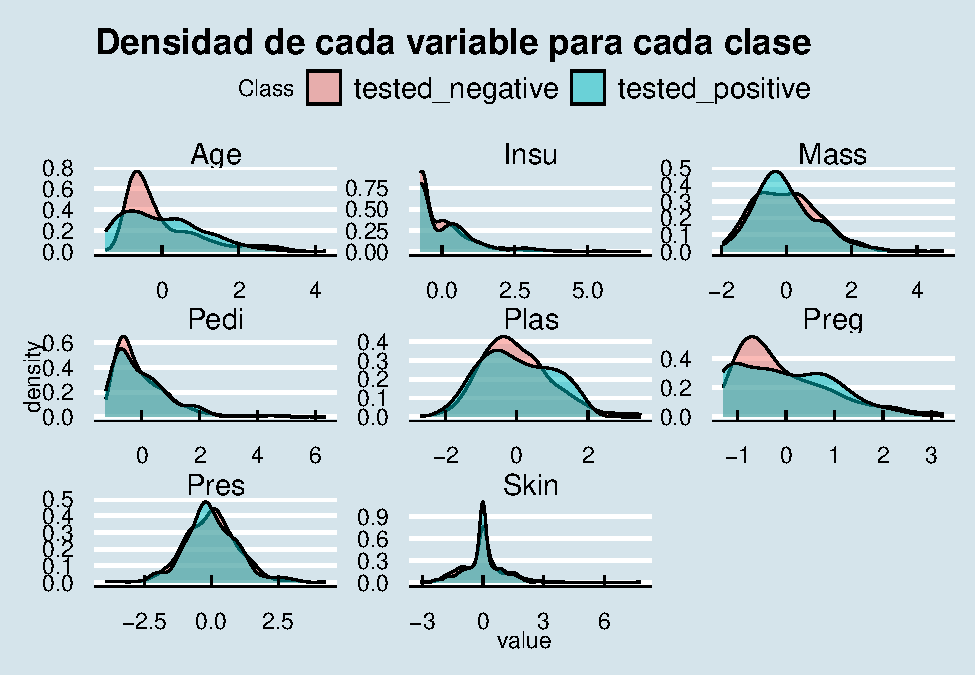
\includegraphics[width=0.75\linewidth]{pima-clasificacion_files/figure-latex/multi_norm_density-1} 

}

\caption{Distribución de cada variable para cada clase}\label{fig:multi_norm_density}
\end{figure}

Dadas las asunciones de LDA, comprobamos que se cumplen. Para ello,
realizamos un test de Shapiro-Wilk para cada variable separada por clase
(Figura \ref{fig:shapiro}) y un test de Barlett para la homocedasticidad
(Figura \ref{fig:barlett}). Vemos que ninguna variable sigue una
distribución normal, aún así, dado que es un requisito y tanto LDA como
QDA son suficientemente robustos sobre algunas desviaciones de la
normalidad, los usaremos. Por otro lado, vemos que la homocedasticidad
se incumple para las variables `Preg', `Plas', `Pedi' e `Insu'.

\begin{figure}

{\centering 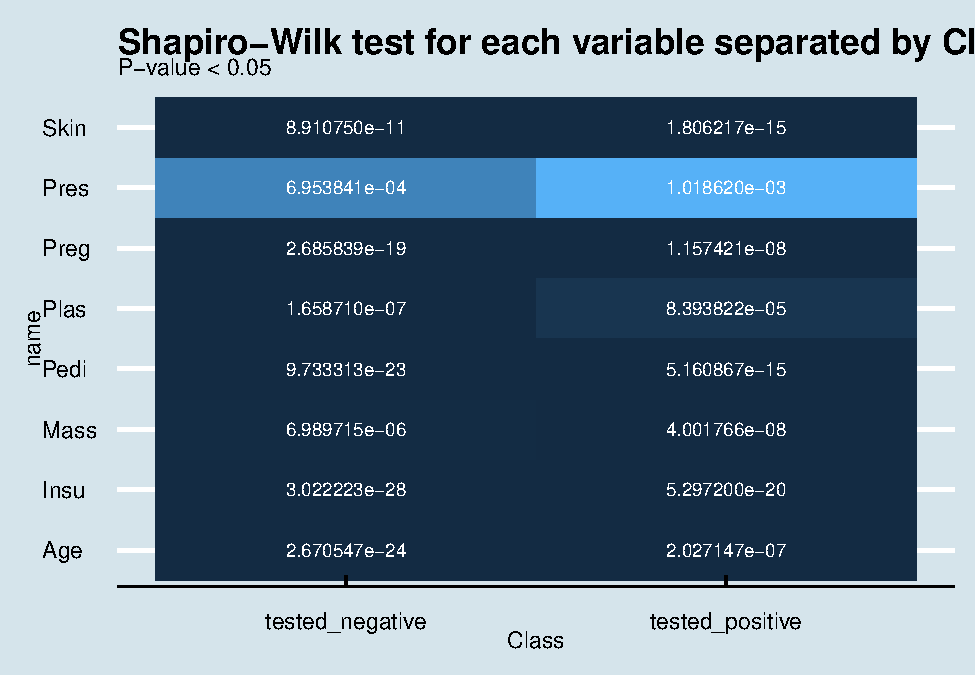
\includegraphics[width=0.75\linewidth]{pima-clasificacion_files/figure-latex/shapiro-1} 

}

\caption{Test de Shapiro-Wilk para cada variable separada por clase}\label{fig:shapiro}
\end{figure}

\begin{figure}

{\centering 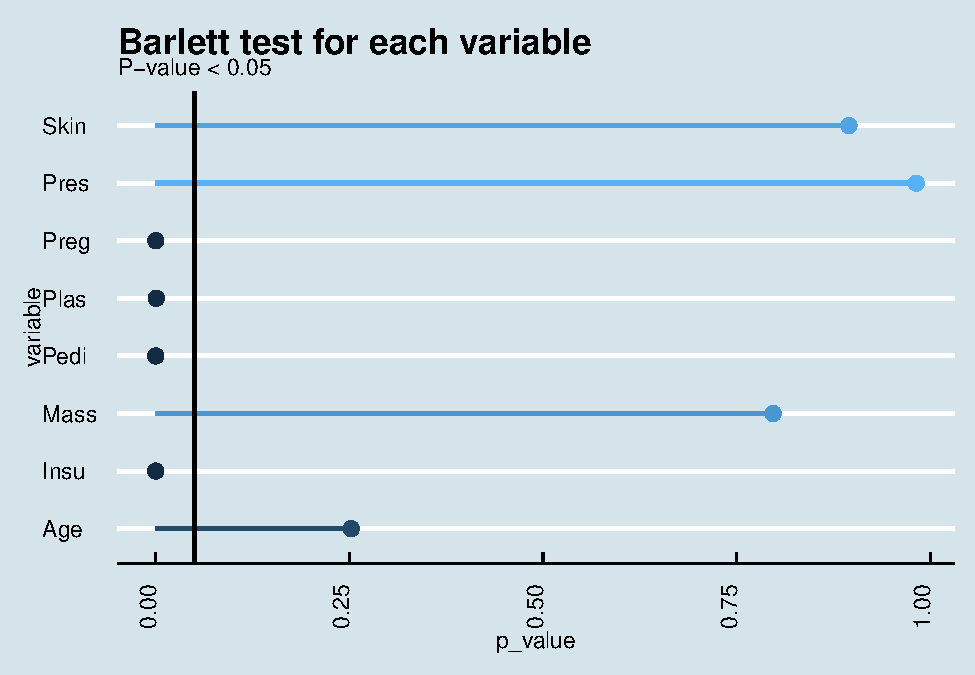
\includegraphics[width=0.5\linewidth]{pima-clasificacion_files/figure-latex/barlett-1} 

}

\caption{Test de Barlett para cada variable separada por clase}\label{fig:barlett}
\end{figure}

Por último nos queda separar el dataset normalizado en train y test
(80\% y 20\% respectivamente) siguiendo la misma metodología que en la
sección de preparación de datos.

Es necesario comprobar el balance de las clases ya que LDA y QDA sufren
de un problema de sesgo hacia la clase mayoritaria. En este caso, vemos
que el dataset está desbalanceado, por lo que haremos un submuestreo de
la clase mayoritaria para equilibrar el dataset del entrenamiento.

\begin{verbatim}
## [1] "Balance de clases (previo):"
\end{verbatim}

\begin{verbatim}
## 
## tested_negative tested_positive 
##             400             215
\end{verbatim}

\begin{verbatim}
## [1] "Balance de clases (posterior):"
\end{verbatim}

\begin{verbatim}
## 
## tested_negative tested_positive 
##             215             215
\end{verbatim}

\hypertarget{lda}{%
\subsubsection{LDA}\label{lda}}

Como se ha mostrado, solo las variables Skin, Pres, Mass y Age no
rechazan la homocedasticidad. Por ello, entrenaremos el modelo solo con
estas variables. Para visualizar la clasificación usaremos la librería
`klaR'. Entrenaremos 2 modelos, uno con el dataset desbalanceado y otro
con el dataset balanceado.

\begin{verbatim}
## [1] "Modelo con dataset desbalanceado:"
\end{verbatim}

\begin{verbatim}
## Call:
## lda(train_lbls ~ Skin + Pres + Mass + Age, data = train)
## 
## Prior probabilities of groups:
## tested_negative tested_positive 
##       0.6504065       0.3495935 
## 
## Group means:
##                         Skin         Pres         Mass         Age
## tested_negative  0.010847726  0.009582014 -0.006401664 0.033640008
## tested_positive -0.009350619 -0.011060642  0.003943845 0.004477913
## 
## Coefficients of linear discriminants:
##             LD1
## Skin -0.7137423
## Pres -0.4211953
## Mass  0.6711865
## Age  -0.4373904
\end{verbatim}

\begin{verbatim}
## [1] "Modelo con dataset balanceado:"
\end{verbatim}

\begin{verbatim}
## Call:
## lda(train_bal_lbls ~ Skin + Pres + Mass + Age, data = train_bal)
## 
## Prior probabilities of groups:
## tested_negative tested_positive 
##             0.5             0.5 
## 
## Group means:
##                         Skin        Pres         Mass         Age
## tested_negative  0.050489335  0.01119844 -0.075128018 0.096928668
## tested_positive -0.009350619 -0.01106064  0.003943845 0.004477913
## 
## Coefficients of linear discriminants:
##             LD1
## Skin -0.7511871
## Pres -0.1577628
## Mass  0.8714400
## Age  -0.3555460
\end{verbatim}

Evaluamos ambos modelos con el conjunto de test. No solo observamos la
precisión sino el recall, ya que nos interesa que el modelo sea capaz de
detectar la clase positiva. Podemos observar como en precisión el modelo
con el dataset desbalanceado tiene mejor rendimiento (65\% frente a
43\%), pero esto se debe a que con el modelo desbalanceado se clasifican
todos los casos como negativos (Recall = 0). En cambio, el modelo con el
dataset balanceado tiene un recall de 0.434, por lo que es capaz de
detectar la clase positiva. Visualizamos la clasificación por cada
conjunto de 2 variables en la Figura \ref{fig:lda}.

\begin{verbatim}
## [1] "Modelo con dataset desbalanceado:"
\end{verbatim}

\begin{verbatim}
## Confusion Matrix and Statistics
## 
##                  Reference
## Prediction        tested_negative tested_positive
##   tested_negative             100              53
##   tested_positive               0               0
##                                           
##                Accuracy : 0.6536          
##                  95% CI : (0.5725, 0.7286)
##     No Information Rate : 0.6536          
##     P-Value [Acc > NIR] : 0.5373          
##                                           
##                   Kappa : 0               
##                                           
##  Mcnemar's Test P-Value : 9.148e-13       
##                                           
##               Precision :     NA          
##                  Recall : 0.0000          
##                      F1 :     NA          
##              Prevalence : 0.3464          
##          Detection Rate : 0.0000          
##    Detection Prevalence : 0.0000          
##       Balanced Accuracy : 0.5000          
##                                           
##        'Positive' Class : tested_positive 
## 
\end{verbatim}

\begin{verbatim}
## [1] "Modelo con dataset balanceado:"
\end{verbatim}

\begin{figure}

{\centering 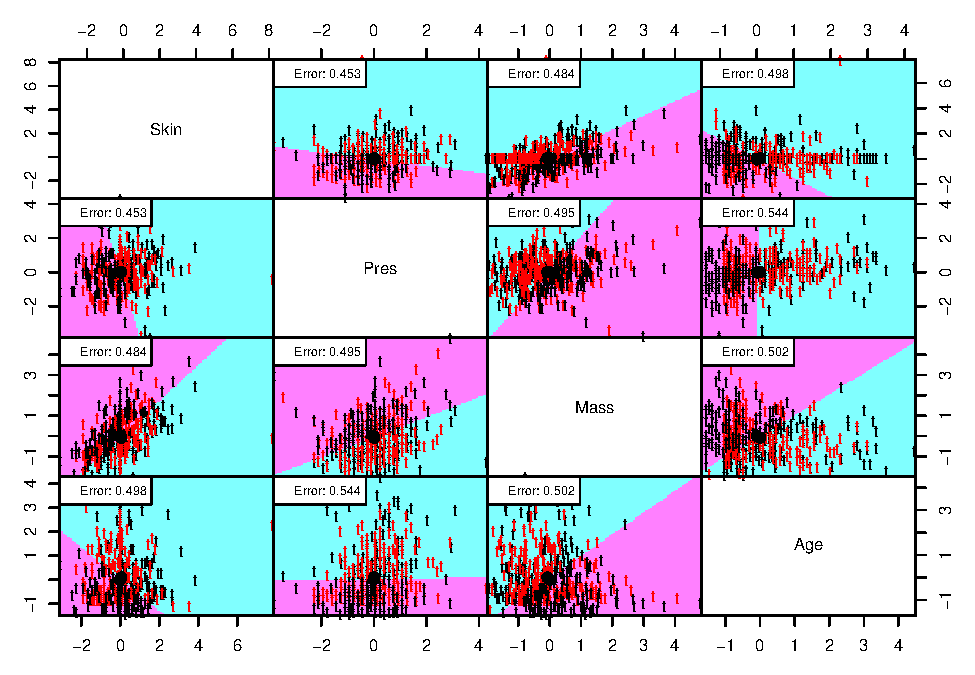
\includegraphics[width=1\linewidth]{pima-clasificacion_files/figure-latex/lda-1} 

}

\caption{Visualización de la clasificación del modelo LDA}\label{fig:lda}
\end{figure}

\hypertarget{qda}{%
\subsubsection{QDA}\label{qda}}

En este apartado usaremos QDA para clasificar los datos. Al igual que en
el apartado anterior, entrenaremos 2 modelos, uno con el dataset
desbalanceado y otro con el dataset balanceado. Siendo que QDA no
requiere que las variables cumplan la homocedasticidad, usaremos todas
las variables para entrenar el modelo.

\begin{verbatim}
## [1] "Modelo con dataset desbalanceado:"
\end{verbatim}

\begin{verbatim}
## Call:
## qda(train_lbls ~ ., data = train)
## 
## Prior probabilities of groups:
## tested_negative tested_positive 
##       0.6504065       0.3495935 
## 
## Group means:
##                        Preg         Plas         Pres         Skin         Insu
## tested_negative  0.01723461 0.0002035090  0.009582014  0.010847726  0.002710759
## tested_positive -0.05982274 0.0004369632 -0.011060642 -0.009350619 -0.012851278
##                         Mass       Pedi         Age
## tested_negative -0.006401664 0.01076950 0.033640008
## tested_positive  0.003943845 0.04428763 0.004477913
\end{verbatim}

\begin{verbatim}
## [1] "Modelo con dataset balanceado:"
\end{verbatim}

\begin{verbatim}
## Call:
## qda(train_bal_lbls ~ ., data = train_bal)
## 
## Prior probabilities of groups:
## tested_negative tested_positive 
##             0.5             0.5 
## 
## Group means:
##                         Preg         Plas        Pres         Skin        Insu
## tested_negative  0.002975206 0.0120453171  0.01119844  0.050489335  0.05484183
## tested_positive -0.059822742 0.0004369632 -0.01106064 -0.009350619 -0.01285128
##                         Mass       Pedi         Age
## tested_negative -0.075128018 0.07003042 0.096928668
## tested_positive  0.003943845 0.04428763 0.004477913
\end{verbatim}

Evaluamos ambos modelos con el conjunto de test. Al igual que en el
apartado anterior, no solo observamos la precisión sino el recall, ya
que nos interesa que el modelo sea capaz de detectar la clase positiva.
Podemos observar como en precisión el modelo con el dataset
desbalanceado tiene mejor rendimiento (64\% frente a 50\%), pero esto se
debe a que con el modelo desbalanceado se clasifican casi todos los
casos como negativos (Recall = 0.09). En cambio, el modelo con el
dataset balanceado tiene un recall de 0.4, por lo que es capaz de
detectar la clase positiva. Visualizamos la clasificación por cada
conjunto de 2 variables en la Figura \ref{fig:qda}.

\begin{verbatim}
## [1] "Modelo con dataset desbalanceado:"
\end{verbatim}

\begin{verbatim}
## Confusion Matrix and Statistics
## 
##                  Reference
## Prediction        tested_negative tested_positive
##   tested_negative              93              48
##   tested_positive               7               5
##                                           
##                Accuracy : 0.6405          
##                  95% CI : (0.5591, 0.7164)
##     No Information Rate : 0.6536          
##     P-Value [Acc > NIR] : 0.667           
##                                           
##                   Kappa : 0.0297          
##                                           
##  Mcnemar's Test P-Value : 6.906e-08       
##                                           
##               Precision : 0.41667         
##                  Recall : 0.09434         
##                      F1 : 0.15385         
##              Prevalence : 0.34641         
##          Detection Rate : 0.03268         
##    Detection Prevalence : 0.07843         
##       Balanced Accuracy : 0.51217         
##                                           
##        'Positive' Class : tested_positive 
## 
\end{verbatim}

\begin{verbatim}
## [1] "Modelo con dataset balanceado:"
\end{verbatim}

\begin{verbatim}
## Confusion Matrix and Statistics
## 
##                  Reference
## Prediction        tested_negative tested_positive
##   tested_negative              55              32
##   tested_positive              45              21
##                                          
##                Accuracy : 0.4967         
##                  95% CI : (0.415, 0.5786)
##     No Information Rate : 0.6536         
##     P-Value [Acc > NIR] : 1.0000         
##                                          
##                   Kappa : -0.0508        
##                                          
##  Mcnemar's Test P-Value : 0.1715         
##                                          
##               Precision : 0.3182         
##                  Recall : 0.3962         
##                      F1 : 0.3529         
##              Prevalence : 0.3464         
##          Detection Rate : 0.1373         
##    Detection Prevalence : 0.4314         
##       Balanced Accuracy : 0.4731         
##                                          
##        'Positive' Class : tested_positive
## 
\end{verbatim}

\begin{figure}

{\centering 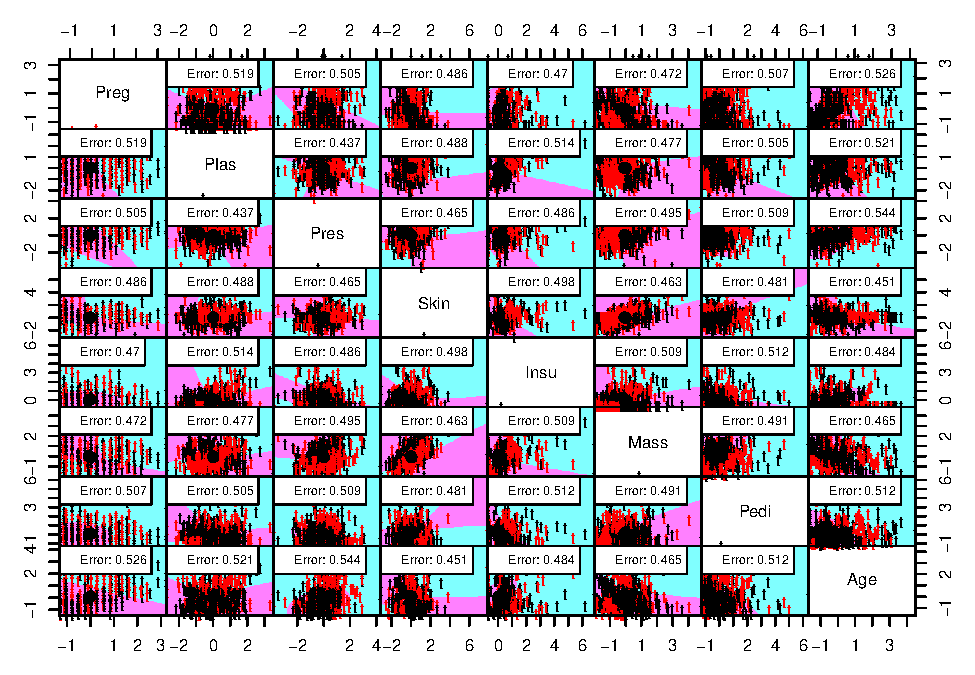
\includegraphics[width=1\linewidth]{pima-clasificacion_files/figure-latex/qda-1} 

}

\caption{Visualización de la clasificación del modelo QDA}\label{fig:qda}
\end{figure}

\hypertarget{fold-cross-validation-1}{%
\subsubsection{10 - fold Cross
Validation}\label{fold-cross-validation-1}}

En este apartado usaremos 10-fold cross validation para evaluar el
rendimiento de los modelos LDA y QDA. Para ello, usaremos las
particiones provistas en el dataset. Se visualizan los resultados por
partición de LDA y QDA en las Figuras \ref{fig:10f_lda} y
\ref{fig:10f_qda} respectivamente.

\begin{figure}

{\centering 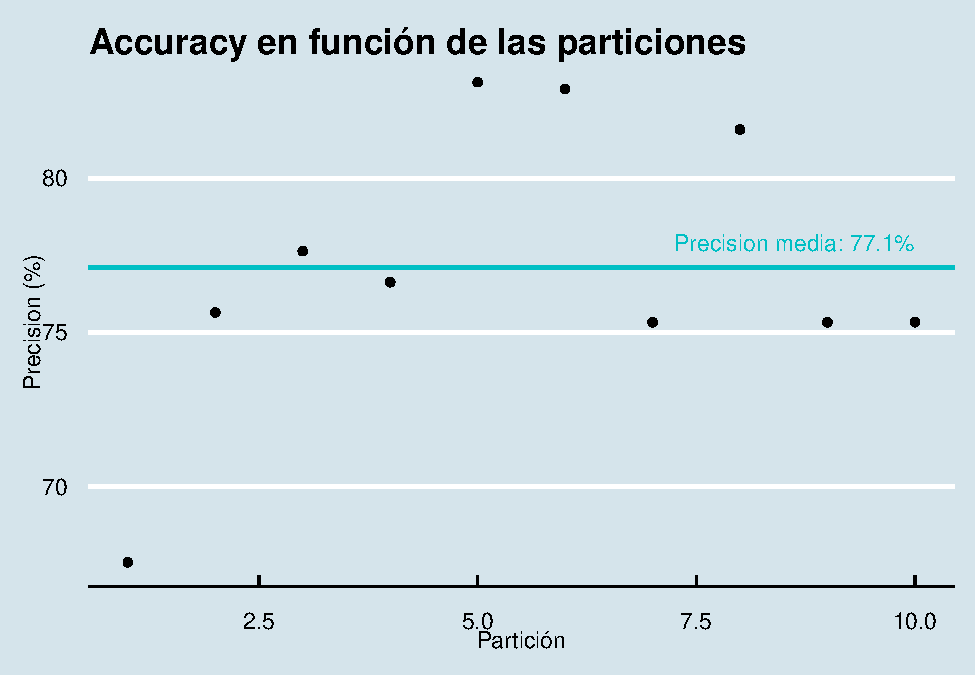
\includegraphics[width=0.5\linewidth]{pima-clasificacion_files/figure-latex/10f_lda-1} 

}

\caption{Accuracy en función de las particiones para LDA}\label{fig:10f_lda}
\end{figure}

\begin{figure}

{\centering 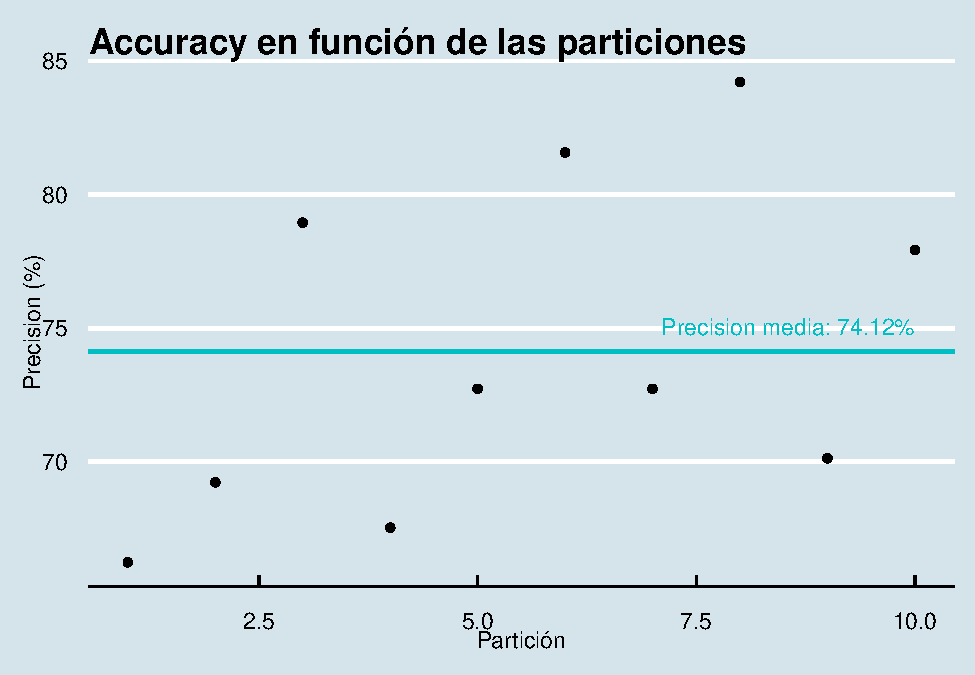
\includegraphics[width=0.5\linewidth]{pima-clasificacion_files/figure-latex/10f_qda-1} 

}

\caption{Accuracy en función de las particiones para QDA}\label{fig:10f_qda}
\end{figure}

\hypertarget{anexo-cuxf3digo-de-la-pruxe1ctica}{%
\section{Anexo : Código de la
práctica}\label{anexo-cuxf3digo-de-la-pruxe1ctica}}

Dado que esto se ha realizado en un archivo de RMarkdown, se puede ver
el código de la práctica en el archivo \texttt{pima-cladificacion.Rmd}
que se encuentra en el repositorio de GitHub.
\href{https://github.com/DanelArias-Dreyton257/DATCOM-Intro/blob/main/pima-clasificacion.Rmd}{Click
aquí}

\end{document}
